\documentclass{article}

% packages
  % basic stuff for rendering math
  \usepackage[letterpaper, top=1in, bottom=1in, left=1in, right=1in]{geometry}
  \usepackage[utf8]{inputenc}
  \usepackage[english]{babel}
  \usepackage{amsmath} 
  \usepackage{amssymb}
  % \usepackage{amsthm}

  % extra math symbols and utilities
  \usepackage{mathtools}        % for extra stuff like \coloneqq
  \usepackage{mathrsfs}         % for extra stuff like \mathsrc{}
  \usepackage{centernot}        % for the centernot arrow 
  \usepackage{bm}               % for better boldsymbol/mathbf 
  \usepackage{enumitem}         % better control over enumerate, itemize
  \usepackage{hyperref}         % for hypertext linking
  \usepackage{fancyvrb}          % for better verbatim environments
  \usepackage{newverbs}         % for texttt{}
  \usepackage{xcolor}           % for colored text 
  \usepackage{listings}         % to include code
  \usepackage{lstautogobble}    % helper package for code
  \usepackage{parcolumns}       % for side by side columns for two column code
  

  % page layout
  \usepackage{fancyhdr}         % for headers and footers 
  \usepackage{lastpage}         % to include last page number in footer 
  \usepackage{parskip}          % for no indentation and space between paragraphs    
  \usepackage[T1]{fontenc}      % to include \textbackslash
  \usepackage{footnote}
  \usepackage{etoolbox}

  % for custom environments
  \usepackage{tcolorbox}        % for better colored boxes in custom environments
  \tcbuselibrary{breakable}     % to allow tcolorboxes to break across pages

  % figures
  \usepackage{pgfplots}
  \pgfplotsset{compat=1.18}
  \usepackage{float}            % for [H] figure placement
  \usepackage{tikz}
  \usepackage{tikz-cd}
  % \usepackage{circuit-tikz}
  \usetikzlibrary{arrows}
  \usetikzlibrary{positioning}
  \usetikzlibrary{calc}
  \usepackage{graphicx}
  \usepackage{caption} 
  \usepackage{subcaption}

  % for tabular stuff 
  \usepackage{dcolumn}

  \usepackage[nottoc]{tocbibind}
  \pdfsuppresswarningpagegroup=1
  \hfuzz=5.002pt                % ignore overfull hbox badness warnings below this limit

% New and replaced operators
  \DeclareMathOperator{\Tr}{Tr}
  \DeclareMathOperator{\Sym}{Sym}
  \DeclareMathOperator{\Span}{span}
  \DeclareMathOperator{\std}{std}
  \DeclareMathOperator{\Cov}{Cov}
  \DeclareMathOperator{\Var}{Var}
  \DeclareMathOperator{\Corr}{Corr}
  \DeclareMathOperator{\pos}{pos}
  \DeclareMathOperator*{\argmin}{\arg\!\min}
  \DeclareMathOperator*{\argmax}{\arg\!\max}
  \newcommand{\ket}[1]{\ensuremath{\left|#1\right\rangle}}
  \newcommand{\bra}[1]{\ensuremath{\left\langle#1\right|}}
  \newcommand{\braket}[2]{\langle #1 | #2 \rangle}
  \newcommand{\qed}{\hfill$\blacksquare$}     % I like QED squares to be black

% Custom Environments
  \newtcolorbox[auto counter, number within=section]{question}[1][]
  {
    colframe = orange!25,
    colback  = orange!10,
    coltitle = orange!20!black,  
    breakable, 
    title = \textbf{Question \thetcbcounter ~(#1)}
  }

  \newtcolorbox[auto counter, number within=section]{exercise}[1][]
  {
    colframe = teal!25,
    colback  = teal!10,
    coltitle = teal!20!black,  
    breakable, 
    title = \textbf{Exercise \thetcbcounter ~(#1)}
  }
  \newtcolorbox[auto counter, number within=section]{solution}[1][]
  {
    colframe = violet!25,
    colback  = violet!10,
    coltitle = violet!20!black,  
    breakable, 
    title = \textbf{Solution \thetcbcounter}
  }
  \newtcolorbox[auto counter, number within=section]{lemma}[1][]
  {
    colframe = red!25,
    colback  = red!10,
    coltitle = red!20!black,  
    breakable, 
    title = \textbf{Lemma \thetcbcounter ~(#1)}
  }
  \newtcolorbox[auto counter, number within=section]{theorem}[1][]
  {
    colframe = red!25,
    colback  = red!10,
    coltitle = red!20!black,  
    breakable, 
    title = \textbf{Theorem \thetcbcounter ~(#1)}
  } 
  \newtcolorbox[auto counter, number within=section]{proof}[1][]
  {
    colframe = orange!25,
    colback  = orange!10,
    coltitle = orange!20!black,  
    breakable, 
    title = \textbf{Proof. }
  } 
  \newtcolorbox[auto counter, number within=section]{definition}[1][]
  {
    colframe = yellow!25,
    colback  = yellow!10,
    coltitle = yellow!20!black,  
    breakable, 
    title = \textbf{Definition \thetcbcounter ~(#1)}
  } 
  \newtcolorbox[auto counter, number within=section]{example}[1][]
  {
    colframe = blue!25,
    colback  = blue!10,
    coltitle = blue!20!black,  
    breakable, 
    title = \textbf{Example \thetcbcounter ~(#1)}
  } 
  \newtcolorbox[auto counter, number within=section]{code}[1][]
  {
    colframe = green!25,
    colback  = green!10,
    coltitle = green!20!black,  
    breakable, 
    title = \textbf{Code \thetcbcounter ~(#1)}
  } 
  \BeforeBeginEnvironment{example}{\savenotes}
  \AfterEndEnvironment{example}{\spewnotes}
  \BeforeBeginEnvironment{lemma}{\savenotes}
  \AfterEndEnvironment{lemma}{\spewnotes}
  \BeforeBeginEnvironment{theorem}{\savenotes}
  \AfterEndEnvironment{theorem}{\spewnotes}
  \BeforeBeginEnvironment{corollary}{\savenotes}
  \AfterEndEnvironment{corollary}{\spewnotes}
  \BeforeBeginEnvironment{definition}{\savenotes}
  \AfterEndEnvironment{definition}{\spewnotes}
  \BeforeBeginEnvironment{exercise}{\savenotes}
  \AfterEndEnvironment{exercise}{\spewnotes}
  \BeforeBeginEnvironment{proof}{\savenotes}
  \AfterEndEnvironment{proof}{\spewnotes}
  \BeforeBeginEnvironment{solution}{\savenotes}
  \AfterEndEnvironment{solution}{\spewnotes}
  \BeforeBeginEnvironment{question}{\savenotes}
  \AfterEndEnvironment{question}{\spewnotes}
  \BeforeBeginEnvironment{code}{\savenotes}
  \AfterEndEnvironment{code}{\spewnotes}

  \definecolor{dkgreen}{rgb}{0,0.6,0}
  \definecolor{gray}{rgb}{0.5,0.5,0.5}
  \definecolor{mauve}{rgb}{0.58,0,0.82}
  \definecolor{lightgray}{gray}{0.93}

  % default options for listings (for code)
  \lstset{
    autogobble,
    frame=ltbr,
    language=C,                           % the language of the code
    aboveskip=3mm,
    belowskip=3mm,
    showstringspaces=false,
    columns=fullflexible,
    keepspaces=true,
    basicstyle={\small\ttfamily},
    numbers=left,
    firstnumber=1,                        % start line number at 1
    numberstyle=\tiny\color{gray},
    keywordstyle=\color{blue},
    commentstyle=\color{dkgreen},
    stringstyle=\color{mauve},
    backgroundcolor=\color{lightgray}, 
    breaklines=true,                      % break lines
    breakatwhitespace=true,
    tabsize=3, 
    xleftmargin=2em, 
    framexleftmargin=1.5em, 
    stepnumber=1
  }

% Page style
  \pagestyle{fancy}
  \fancyhead[L]{}
  \fancyhead[C]{Muchang Bahng}
  \fancyhead[R]{Spring 2024} 
  \fancyfoot[C]{\thepage / \pageref{LastPage}}
  \renewcommand{\footrulewidth}{0.4pt}          % the footer line should be 0.4pt wide
  \renewcommand{\thispagestyle}[1]{}  % needed to include headers in title page

\begin{document}

\title{Advanced Machine Learning}
\author{Muchang Bahng}
\date{Spring 2024}

\maketitle
\tableofcontents
\pagebreak

Machine learning in the 1980s have been focused on developing rigorous theory of learning algorithms, and the field has been dominated by statisticians. They strived to develop the theoretical foundation of algorithms that can be implemented and applied to real-world data. These days, machine learning is more of an engineering discipline than a science. With the advent of deep learning, the theory behind these black box algorithms has slowed down, but their applications have exploded. It is now a field of trying out a bunch of things and sticking to what works. These set of notes are for the former theory, while my deep learning notes are for the latter. It is covered in a separate set of notes since a lot of space is needed to talk about recent developments and architectures (e.g. RCNN, YOLO, LSTMs, Transformers, VAEs, GANs, etc.). We will focus more on establishing the theoretical foundations of most learning algorithms and analyze interpretable algorithms. 

I've spent a good amount of time trying to create a map of machine learning, but after rewriting these notes multiple times. I've come to the conclusion that it is impossible to create a nice chronological map of machine learning. Like math, you keep on revisiting the same topics over and over again, but at a higher level, and it's not as simple to organize everything into parametric vs nonparametric\footnote{K nearest neighbors is a nonparameteric model given that the data is not fixed. When the data is fixed, then our function search space is finite.}, supervised vs unsupervised\footnote{There are semi-supervised or weakly supervised models, and models like autoencoders use a supervised algorithm without any labels.}, or discriminative vs generative models.\footnote{Using Bayes rule, we can always reduce generative models into discriminative models.} Therefore, this is what I recommend. 

\begin{enumerate}
  \item If you are new to machine learning, go over my notes on Stanford CS229, which simply covers basic algorithms and their implementation. 
  \item Then go over my supervised and unsupervised machine learning notes to get a better grasp of these algorithms, with a bit of theory behind them. 
  \item Now you can learn the deeper theory of machine learning. This is what these notes are for. 
\end{enumerate}
You should know measure (probability) theory, a bit of functional analysis, and some statistics. I will reintroduce all the necessary definitions in a way that is as general as possible, as we move along. 


\section{Statistical Learning Theory} 

  \subsection{Concentration Inequalities}

  \subsection{Minimax Theory}

  \subsection{Empirical Risk Minimization} 

    Unlike unsupervised learning, which comes in many different shapes and forms (anomaly detection, feature extraction, density estimation, dimensionality reduction, etc.), supervised learning comes in a much cleaner format. 
    \begin{enumerate}
      \item We start off with a general probability space $(\Omega, \mathcal{F}, \mathbb{P})$. This is our model of the world and everything that we are interested in. 

      \item A measurable function $X: \Omega \rightarrow \mathcal{X}$ extracts a set of features, which we call the \textbf{covariates} and induces a probability measure on $\mathcal{X}$, say $\mathbb{P}_X$. 

      \item Another measurable function $Y: \Omega \rightarrow \mathcal{Y}$ extracts another set of features called the \textbf{labels} and induces another probability measure on $\mathcal{Y}$, the \textbf{label set}, say $\mathbb{P}_Y$. 

      \item At this point the function $X \times Y$ is all we are interested in, and we throw away $\Omega$ since we only care about the distribution over $\mathcal{X} \times \mathcal{Y}$. 

      \item We model the generation of data from $\Omega$ by sampling $N$ samples from $\mathbb{P}_{X \times Y}$, which we assume to be iid (this assumption will be relaxed later). This gives us the \textbf{dataset} 
        \[\mathcal{D} = \{(\mathbf{x}^{(i)}, \mathbf{y}^{(i)}) \}_{i=1}^N\]

      \item We want to learn a prediction rule, or a \textbf{hypothesis function} $h: \mathcal{X} \rightarrow \mathcal{Y}$, which is searched within a set of functions $\mathcal{H}$, called a \textbf{hypothesis class}. 

      \item We want a measure of how good the hypothesis is. This can be measured with some custom loss function $L: \mathcal{X} \times \mathcal{Y} \times \mathcal{H} \rightarrow \mathbb{R}_+$ which measures the ``loss" of a function $h \in \mathcal{H}$ on the data point $(x, y)$. This results in us being able to define the \textbf{error} of our hypothesis to be 
        \[E(h) \coloneqq \int_{\mathcal{X} \times \mathcal{Y}} L (x, y, h) \,d\mathbb{P}_{X \times Y}\]
    \end{enumerate}

    The problem is that we don't know the distribution of $\mathbb{P}_{X \times Y}$, and so we must resort to our dataset, which yields the empirical error.  

  \subsection{Decision Theory}

    How do we choose our loss functions? 

\section{Low Dimensional Linear Regression}

    Low dimensional linear regression is what statisticians worked in back in the early days, where data was generally low dimensional.\footnote{Quoting Larry Wasserman, even 5 dimensions was considered high and 10 was considered massive. } Generally, we had $d < n$, but these days, we are in the regime where $d > n$. For example, in genetic data, you could have a sample of $n = 100$ people but each of them have genetic sequences at $d = 10^6$. When the dimensions become high, the original methods of linear regression tend to break down, which is why I separate low and high dimensional linear regression. 

    In here, we start with \textbf{multiple linear regression}, which assumes that we have several covariates and one response. If we extend this to multiple responses (i.e. a response vector), this is called \textbf{multivariate linear regression}. The simple case for one response is called \textbf{simple linear regression}, and we will mention some nice formulas and intuition that come out from working with this. 

  \subsection{Construction}

    \begin{definition}[Multiple Linear Regression]
      Given a dataset $\mathcal{D} = \{(\mathbf{x}^{(i)}, y^{(i)})\}_{i=1}^N$, where $\mathbf{x}^{(i)} \in \mathbb{R}^d$ and $y^{(i)} \in \mathbb{R}$, the multiple linear regression model is 
      \begin{equation}
        y = \beta^T x + \epsilon
      \end{equation}
      with the following assumptions: 
      \begin{enumerate}
        \item \textit{Weak exogeneity}: the covariates are observed without error.
        \item \textit{Linearity}: the mean of the variate is a linear combination of the parameters and the covariates.
        \item \textit{Gaussian errors}: the errors are Gaussian.\footnote{We can relax this assumption when we get into generalized linear models, and in most cases we assume some closed form of the error for computational convenience, like when computing the maximum likelihood.}
        \item \textit{Homoscedasticity}: the errors (the observations of $Y$) have constant variance. 
        \item \textit{Independence of errors}: The errors are uncorrelated.
        \item \textit{No multicollinearity}: more properly, the lack of perfect multicollinearity. Assume that the covariates aren't perfectly correlated.\footnote{This is the assumption that breaks down in high dimensional linear regression.} 
      \end{enumerate}
    \end{definition}

    In order to check multicollinearity, we compute the correlation matrix. 

    \begin{definition}[Correlation Matrix]
      The correlation matrix of random variables $X_1, \ldots, X_d$ is 
      \[\mathbf{C}_{ij} = \Corr(X_i, X_j) = \frac{\Cov(X_i, X_j)}{\sigma_{X_i} \sigma_{X_j}}\]
      given that $\sigma_{X_i} \sigma_{X_j} > 0$. Clearly, the diagonal entries are $1$, but if there are entries that are very close to $1$, then we have multicollinearity. 
    \end{definition}

    Assume that two variables are perfectly correlated. Then, there would be pairs of parameters that are indistinguishable if moved in a certain linear combination. This means that the variance of $\hat{\boldsymbol{\beta}}$ will be very ill conditioned, and you would get a huge standard error in some direction of the $\beta_i$'s. We can fix this by making sure that the data is not redundant and manually removing them, standardizing the variables, making a change of basis to remove the correlation, or just leaving the model as it is. 

    If these assumptions don't hold, 
    \begin{enumerate}
      \item \textit{Weak exogeneity}: the sensitivity of the model can be tested to the assumption of weak exogeneity by doing bootstrap sampling for the covariates and seeing how the sampling affects the parameter estimates.
      Covariates measured with error used to be a difficult problem to solve, as they required errors-in-variables models, which have very complicated likelihoods. In addition, there is no universal fitting library to deal with these. But nowadays, with the availability of Markov Chain Monte Carlo (MCMC) estimation through probabilistic programming languages, it is a lot easier to deal with these using Bayesian hierarchical models (or multilevel models, or Bayesian graphical models---these have many names).

      \item \textit{Linearity}: the linear regression model only assumes linearity in the parameters, not the covariates. Therefore you could build a regression using non-linear transformations of the covariates, for instance,
      \begin{equation}
        Y = X_1 \beta_1 + X_1^2 \beta_2 + \log(X_1) \beta_3
      \end{equation}
      If you need to further relax the assumption, you are better off using non-linear modelling. 

      \item \textit{Constant variance}: the simplest fix is to do a variance-stabilising transformation on the data. Assuming a constant coefficient of variation rather than a constant mean could also work. Some estimation libraries (such as the \verb+glm+ package in R) allow specifying the variance as a function of the mean.

      \item \textit{Independence of errors}: this is dangerous because in the financial world things are usually highly correlated in times of crisis. The most important thing is to understand how risky this assumption is for your setting. If necessary, add a correlation structure to your model, or do  a multivariate regression. Both of these require significant resources to estimate parameters, not only in terms of computational power but also in the amount of data required.

      \item \textit{No multicollinearity}: If the covariates are correlated, they can still be used in the regression, but numerical problems might occur depending on how the fitting algorithms invert the matrices involved. The t-tests that the regression produces can no longer be trusted. All the covariates must be included regardless of what their significance tests say.
      A big problem with multicollinearity, however, is over-fitting.
      Depending on how bad the situation is, the parameter values might have huge uncertainties around them, and if you fit the model using new data their values might change significantly.\footnote{I suggest reading this Wikipedia article on multicollinearity, as it contains useful information: \url{https://en.wikipedia.org/wiki/Multicollinearity}} Multicollinearity is a favourite topic of discussion for quant interviewers, and they usually have strong opinions about how it should be handled. The model's intended use will determine how sensitive it is to ignoring the error distribution. In many cases, fitting a line using least-squares estimation is equivalent to assuming errors have a normal distribution. If the real distribution has heavier tails, like the t-distribution, how risky will it make decisions based on your outputs? One way to address this is to use a technique like robust-regression. Another way is to think about the dynamics behind the problem and which distribution would be best suited to model them---as opposed to just fitting a curve through a set of points.
    \end{enumerate}

  \subsection{Least Squares}

    Given the design matrix $\mathbf{X}$, we can present the linear model in vectorized form: 

    \[\mathbf{Y} = \mathbf{X} \boldsymbol{\beta} + \boldsymbol{\epsilon}, \; \boldsymbol{\epsilon} \sim N(\mathbf{0}, \sigma^2 \mathbf{I})\]

    The errors can be written as $\boldsymbol{\epsilon} = \mathbf{Y} - \mathbf{X} \boldsymbol{\beta}$, and you have the following total sum of squared errors: 

    \[S(\boldsymbol{\beta}) = \boldsymbol{\epsilon}^T \boldsymbol{\epsilon} = (\mathbf{Y} - \mathbf{X} \boldsymbol{\beta})^T (\mathbf{Y} - \mathbf{X} \boldsymbol{\beta})\]

    We want to find the value of $\boldsymbol{\beta}$ that minimizes the sum of squared errors. In order to do this, remember the following matrix derivative rules when differentiating with respect to vector $\mathbf{x}$. 
    \begin{enumerate}
      \item $\mathbf{x}^T \mathbf{A} \mapsto \mathbf{A}$
      \item $\mathbf{x}^T \mathbf{A} \mathbf{x} \mapsto 2 \mathbf{A} \mathbf{x}$
    \end{enumerate}
    Now this should be easy. 
    \begin{align*}
        S(\boldsymbol{\beta}) & = \mathbf{Y}^T \mathbf{Y} - \boldsymbol{\beta}^T \mathbf{X}^T \mathbf{Y} - \mathbf{Y}^T \mathbf{X} \boldsymbol{\beta} + \boldsymbol{\beta}^T \mathbf{X}^T \mathbf{X} \boldsymbol{\beta} \\
        & = \mathbf{Y}^T \mathbf{Y} - 2 \mathbf{Y}^T \mathbf{X} \boldsymbol{\beta} + \boldsymbol{\beta}^T \mathbf{X}^T \mathbf{X} \boldsymbol{\beta} \\
        \frac{\partial}{\partial \boldsymbol{\beta}} S(\boldsymbol{\beta}) & = - 2 \mathbf{X}^T \mathbf{Y} + 2 \mathbf{X}^ \mathbf{X} \boldsymbol{\beta}
    \end{align*}
    and setting it to $\mathbf{0}$ gives 
    \[2 \mathbf{X}^T \mathbf{X} \boldsymbol{\beta} - 2 \mathbf{X}^T \mathbf{Y} = 0 \implies \mathbf{X}^T \mathbf{X} \boldsymbol{\beta} = \mathbf{X}^T \mathbf{Y}\]
    and the variance of $\boldsymbol{\beta}$, by using the fact that $\Var[\mathbf{A} \mathbf{X}] = \mathbf{A} \Var[X] \mathbf{A}^T$, is
    \[\Var(\hat{\boldsymbol{\beta}}) =
     (\mathbf{X}^{\prime} \mathbf{X})^{-1} \mathbf{X}^{\prime}
     \;\sigma^2 \mathbf{I} \; \mathbf{X}  (\mathbf{X}^{\prime} \mathbf{X})^{-1}
    = \sigma^2 (\mathbf{X}^{\prime} \mathbf{X})^{-1} (\mathbf{X}^{\prime}
     \mathbf{X})  (\mathbf{X}^{\prime} \mathbf{X})^{-1}
    = \sigma^2  (\mathbf{X}^{\prime} \mathbf{X})^{-1}\]
    But we don't know the true $\sigma^2$, so we estimate it with $\hat{\sigma}^2$ by taking the variance of the residuals. Therefore, we have 
    \begin{align*}
        \boldsymbol{\beta} & = (\mathbf{X}^T \mathbf{X})^{-1} \mathbf{X}^T \mathbf{Y} \in \mathbb{R}^d \\
        \Var(\hat{\boldsymbol{\beta}}) & = \hat{\sigma}^2 (\mathbf{X}^T \mathbf{X})^{-1} \in \mathbb{R}^{d \times d}
    \end{align*}

    \begin{example}
    What happens if you copy your data in OLS? In this case, our MLE estimate becomes 
    \begin{align*}
        \left(\begin{pmatrix}X \\ X \end{pmatrix}^T \begin{pmatrix} X \\ X \end{pmatrix} \right )^{-1} & \begin{pmatrix} X \\ X  \end{pmatrix}^T \begin{pmatrix} Y \\ Y  \end{pmatrix}  =\\
    & = (X^T X + X^T X)^{-1} (X^T Y + X^T Y ) = (2 X^T X)^{-1} 2 X^T Y = \hat{\beta}
    \end{align*}
    and our estimate is unaffected. However, the variance shrinks by a factor of $2$ to 
    \[\frac{\sigma^2}{2} (\mathbf{X}^T \mathbf{X})^{-1}\]
    A consequence of that is that confidence intervals will shrink with a factor of $1/\sqrt{2}$. The reason is that we have calculated as if we still had iid data, which is untrue. The pair of doubled values are obviously dependent and have a correlation of $1$. 
    \end{example}

  \subsection{Likelihood Estimation}

    Given a dataset $\mathcal{D} = \{(x^{(i)}, y^{(i)})\}_{i=1}^N$, our likelihood is 
    \[L(\theta ; \mathcal{D}) = \prod_{i=1}^N p(y^{(i)} \mid x^{(i)}; \theta) = \prod_{i=1}^N \frac{1}{\sqrt{2 \pi \sigma^2}} \exp \bigg( -\frac{(y^{(i)} - \theta^T x^{(i)})^2}{2 \sigma^2} \bigg)\]
    We can take its negative log, remove additive constants, and scale accordingly to get 
    \begin{align*}
        \ell (\theta) & = -\frac{N}{2} \ln{\sigma^2} - \frac{N}{2} \ln(2 \pi) + \frac{1}{2 \sigma^2} \sum_{i=1}^N \big(y^{(i)} - \boldsymbol{\theta}^T \mathbf{x}^{(i)} \big)^2 \\
        & =\frac{1}{2} \sum_{i=1}^N \big(y^{(i)} - \boldsymbol{\theta}^T \mathbf{x}^{(i)} \big)^2 
    \end{align*}
    which then corresponds to minimizing the sum of squares error function. Taking the gradient of this log likelihood w.r.t. $\theta$ gives 
    \[\nabla_\theta \ell (\theta) = \sum_{i=1}^N ( y^{(i)} - \theta^T x^{(i)}) x^{(i)} \]
    and running gradient descent over a minibatch $M \subset \mathcal{D}$ gives 
    \begin{align*}
        \theta & = \theta - \eta \nabla_\theta \ell (\theta) \\
        & = \theta - \eta \sum_{(x, y) \in M} (y - \theta^T x) x
    \end{align*}
    This is guaranteed to converge since $\ell(\theta)$, as the sum of convex functions, is also convex. 

    Note that since we can solve this in closed form, by setting the gradient to $0$, we have 
    \[0 = \sum_{n=1}^N y^{(n)} \boldsymbol{\phi}(\mathbf{x}^{(n)})^T - \mathbf{w}^T \bigg( \sum_{n=1}^N \boldsymbol{\phi}(\mathbf{x}^{(n)}) \boldsymbol{\phi}(\mathbf{x}^{(n)})^T \bigg)\]
    which is equivalent to solving the least squares equation 
    \[\mathbf{w}_{ML} = ( \boldsymbol{\Phi}^T \boldsymbol{\Phi})^{-1} \boldsymbol{\Phi}^T \mathbf{Y}\]
    Note that if we write out the bias term out explicitly, we can see that it just accounts for the translation (difference) between the average of the outputs $\bar{y} = \frac{1}{N} \sum_{n=1}^N y_n$ and the average of the basis functions $\bar{\phi_j} = \frac{1}{N} \sum_{n=1}^N \phi_j (\mathbf{x}^{(n)})$. 
    \[w_0 = \bar{y} - \sum_{j=1}^{M-1} w_j \bar{\phi_j}\]
    We can also maximize the log likelihood w.r.t. $\sigma^2$, which gives the MLE 
    \[\sigma^2_{ML} = \frac{1}{N} \sum_{n=1}^N \big( y^{(n)} - \mathbf{w}^T_{ML} \boldsymbol{\phi}(\mathbf{x}^{(n)}) \big)^2\]

  \subsection{Weighted Least Squares}


  \subsection{Simple Linear Regression}

    The simple linear regression is the special case of the linear regression with only one covariate. 
    \[y = \alpha + x \beta\]
    which is just a straight line fit. Interviewers like this model for its aesthetically pleasing theoretical properties. A few of them are described here, beginning with parameter estimation. For $n$ pairs of $(x_i, y_i)$, 
    \[y_i = \alpha + \beta x_i + \epsilon_i\]
    To minimize the sum of squared errors 
    \[\sum_{i} \epsilon_i^2 = \sum_{i} (y_i - \alpha - \beta x_i)^2\]
    Taking the partial derivatives w.r.t. $\alpha$ and $\beta$ and setting them equal to $0$ gives 
    \begin{align*}
        &\sum_i (y_i - \hat{\alpha} - \hat{\beta} x_i) = 0 \\
        &\sum_i (y_i - \hat{\alpha} - \hat{\beta} x_i) x_i = 0
    \end{align*}
    From just the first equation, we can write 
    \[n \bar{y} = n \hat{\alpha} + n \hat{\beta} \bar{x} \implies y = \hat{\alpha} + \hat{\beta} \bar{x} \implies \hat{\alpha}  = \bar{y} - \hat{\beta} \bar{x} \]
    The second equation gives 
    \[\sum_{i} x_i y_i = \hat{\alpha} n \bar{x} + \hat{\beta} \sum_{i} x_i^2\]
    and substituting what we derived gives 
    \begin{align*}
        \sum_{i} x_i y_i & = (\bar{y} - \hat{\beta} \bar{x}) n \bar{x} + \hat{\beta} \sum_i x_i^2 \\
        & = n \bar{x} \bar{y} + \hat{\beta} \bigg( \Big(\sum_i x_i^2 \Big) - n \bar{x}^2 \bigg)
    \end{align*}
    and so we have 
    \[\hat{\beta} = \frac{ \big( \sum_i x_i y_i \big) - n \bar{x}\bar{y}}{\big( \sum x_i^2 \big) - n \bar{x}^2} = \frac{ \sum_i x_i y_i - \bar{x} y_i}{\sum x_i^2 - \bar{x} x_i} = \frac{ \sum_i (x_i - \bar{x}) y_i}{\sum_i (x_i - \bar{x}) x_i}\]
    Now we can use the identity
    \begin{align*}
        \sum_{i} (x_i - \bar{x}) (y_i - \bar{y}) & = \sum_i y_i (x_i - \bar{x}) = \sum_i x_i (y_i - \bar{y}) 
    \end{align*}
    to substitute both the numerator and denominator of the equation to 
    \begin{align*}
        \hat{\beta} & = \frac{\sum_i (x_i - \bar{x}) (y_i - \bar{y})}{\sum_i (x_i - \bar{x})^2} = \frac{\mathrm{cov}(x, y)}{\mathrm{var}(x)} = \rho_{xy} \frac{s_y}{s_x}
    \end{align*}
    where $\rho_{xy}$ is the correlation between $x$ and $y$, and the variance and covariance represent the sample variance and covariance (indicated in lower case letters). Therefore, the correlation coefficient $\rho_{xy}$ is precisely equal to the slope of the best fit line when $x$ and $y$ have been standardized first, i.e. $s_x = s_y = 1$. 

    \begin{example}
    Say that we are fitting $Y$ onto $X$ in a simple regression setting with MLE $\beta_1$, and now we wish to fit $X$ onto $Y$. How will the MLE slope change? We can see that 
    \[\beta_1 = \rho \frac{s_y}{s_x} , \;\; \beta_2 = \rho \frac{s_x}{s_y}\]
    and so 
    \[\beta_2 = \rho^2 \frac{1}{\rho} \frac{s_x}{s_y} = \rho^2 \frac{1}{\beta_1} = \beta_1 \frac{\mathrm{var}(x)}{\mathrm{var}(y)}\]
    The reason for this is because regression lines don't necessarily correspond to one-to-one to a casual relationship. Rather, they relate more directly to a conditional probability or best prediction. 
    \end{example}

    The \textbf{coefficient of determination} $R^2$ is a measure tells you how well your line fits the data. When you have your $y_i$'s, their deviation around its mean is captured by the sample variance $s^2_y = \sum_i (y_i - \bar{y})^2$. When we fit our line, we want the deviation of $y_i$ around our predicted values $\hat{y}_i$, i.e. our sum of squared loss $\sum_i (y_i - \hat{y}_i)^2$, to be lower. Therefore, we can define 
    \[R^2 = 1 - \frac{\mathrm{MSE Loss}}{\mathrm{var}(y)} = 1 - \frac{\sum_i (y_i - \hat{y}_i)^2}{\sum_i (y_i - \bar{y})^2}\]
    In simple linear regression, we have 
    \[R^2 = \rho_{yx}^2\]
    An $R^2$ of $0$ means that the model does not improve prediction over the mean model and $1$ indicates perfect prediction. However, a drawback of $R^2$ is that it can increase if we add predictors to the regression model, leading to a possible overfitting. 

    \begin{theorem}
    The residual sum of squares (RSS) is equal to the a proportion of the variance of the $y_i$'s. 
    \[\mathrm{RSS} = \sum (y_i - \hat{y}_i)^2 = (1 - \rho^2) \sum (y_i - \bar{y})^2 \]
    \end{theorem}

  \subsection{Significance Tests}

    \subsubsection{T Test}

      Given some multilinear regression problem where we must estimate $\boldsymbol{\beta} \in \mathbb{R}^{D + 1}$ ($D$ coefficients and $1$ bias), we must determine whether there is actually a linear relationship between the $x$ and $y$ variables in our dataset $\mathcal{D}$. Say that we have a sample of $N$ points $\mathcal{D} = \{(x_n, y_n)\}_{n=1}^N$. Then, for each ensemble of datasets $\mathcal{D}$ that we sample from the distribution $(X \times Y)^N$, we will have some estimator $\boldsymbol{\beta}$ for each of them. This will create a sampling distribution of $\boldsymbol{\beta}$'s where we can construct our significance test on. 

      So what should our sampling distribution of $\hat{\boldsymbol{\beta}}$ be? It is clearly normal since it is just a transformation of the normally distributed $Y$: $\hat{\boldsymbol{\beta}} \sim N (\boldsymbol{\beta}, \sigma^2 (X^T X)^{-1})$. Therefore, only considering one element $\beta_i$ here, 
      \[\frac{\hat{\beta}_i - \beta_i}{\sigma \sqrt{ (X^T X)^{-1}_{ii}}} \sim N(0, 1)\]
      But the problem is that we don't know the true $\sigma^2$, and we are estimating it with $\hat{\sigma}^2$. If we knew the true $\sigma^2$ then this would be a normal, but because of this estimate, our normalizing factor is also random. It turns out that the residual sum of squares (RSS) for a multiple linear regression
      \[\sum_{i} (y_i - x_i^T \beta)^2 \]
      follows a $\chi^2_{n-d}$ distribution. Additionally from the $\chi^2$ distribution of RSS we have 
      \[\frac{(n - d) \hat{\sigma}^2}{\sigma^2} \sim \chi^2_{n-d}\]
      where we define $\hat{\sigma}^2 = \frac{\mathrm{RSS}}{n-d}$ which is an unbiased estimator for $\sigma^2$. Now there is a theorem that says that if you divide a $N(0, 1)$ distribution by a $\chi^2_k / k$ distribution (with $k$ degrees of freedom), then it gives you a $t$-distribution with the same degrees of freedom. Therefore, we divide 
      \[\frac{\frac{\hat{\beta}_i - \beta_i}{\sqrt{ (X^T X)^{-1}_{ii}}}}{\hat{\sigma}} = \frac{ \sigma \sim N(0, 1)}{\sigma \chi^2_{n-d} / (n-d)} = \frac{\sim N(0, 1)}{\chi^2_{n-d} / (n-d)} = t_{n-d}\]
      where the standard error of the distribution is 
      \[\mathrm{SE}(\hat{\beta}_i) = \sigma_{\hat{\beta}_i} = \sigma \sqrt{(X^T X)^{-1}_{ii}} \]

      In ordinary linear regression, we have the null hypothesis $h_0 : \beta_i = 0$ and the alternative $h_a : \beta_i \neq 0$ for a two sided test or $h_a : \beta_i > 0$ for a one sided test. Given a certain significance level, we compute the critical values of the $t$-distribution at that level and compare it with the test statistic 
      \[t = \frac{\hat{\beta} - 0}{\mathrm{SE}(\hat{\beta})}\]

      Now given our $\beta$, how do we find the standard error of it? Well this is just the variance of our estimator $\boldsymbol{\beta}$, which is $\hat{\sigma}^2 (\mathbf{X}^T \mathbf{X})^{-1}$, where $\hat{\sigma}^2$ is estimated by taking the variance of the residuals $\epsilon_i$. When there is a single variable, the model reduces to 
      \[y = \beta_0 + \beta_1 x + \epsilon\]
      and 
      \[\mathbf{X} = \left(
      \begin{array}{cc}
      1 & x_1 \\
      1 & x_2 \\
      \vdots & \vdots \\
      1 & x_n
      \end{array}
      \right), \qquad \boldsymbol{\beta} = \left(
      \begin{array}{c}
      \beta_0 \\ \beta_1 
      \end{array}
      \right)\]
      and so 
      \[(\mathbf{X}^{\prime} \mathbf{X})^{-1} = \frac{1}{n\sum x_i^2 - (\sum x_i)^2} 
      \left(
      \begin{array}{cc}
      \sum x_i^2 & -\sum x_i \\
      -\sum x_i  & n
      \end{array}
      \right)\]
      and substituting this in gives 
      \[\sqrt{\widehat{\textrm{Var}}(\hat{\beta_1})} = \sqrt{[\hat{\sigma}^2  (\mathbf{X}^{\prime} \mathbf{X})^{-1}]_{22}} = \sqrt{\frac{\hat{\sigma}^2}{\sum x_i^2 - (\sum x_i)^2}} = \sqrt{\frac{\hat{\sigma}^2}{\sum (x_i - \bar{x}_i)^2}}\]

      \begin{example}
      Given a dataset 
      \begin{verbatim}
      Hours Studied for Exam 20 16 20 18 17 16 15 17 15 16 15 17 16 17 14
      Grade on Exam 89 72 93 84 81 75 70 82 69 83 80 83 81 84 76
      \end{verbatim}
      The hypotheses are $h_0 : \beta = 0$ and $h_a : \beta \neq 0$, and the degrees of freedom for the $t$-test is $df = N - (D + 1) = 13$, where $N = 15$ is the number of datapoints and $D = 1$ is the number of coefficients (plus the 1 bias term). The critical values is $\pm 2.160$, which can be found by taking the inverse CDF of the $t$-distribution evaluated at $0.975$. 

      Now we calculate the $t$ score. We have our estimate $\beta_1 = 3.216, \beta_0 = 26.742$, and so we calculate 
      \begin{align*}
          \hat{\sigma}^2 & = \frac{1}{15} \sum_{i=1}^{15} \big( y_i - (3.216 x_i + 26.742) \big) = 13.426 \\
          \sum_{i} (x_i - \hat{x}_i)^2 & = 41.6 
      \end{align*}
      and therefore, we can compute 
      \[t = \frac{\beta_1}{\sqrt{\hat{\sigma}^2 /  \sum_{i} (x_i - \hat{x}_i)^2}} = \frac{3.216}{\sqrt{13.426/41.6}} = 5.661\]
      and therefore, this is way further than our critical value of $2.16$, meaning that we reject the null hypothesis. 
      \end{example}

      Note that when multicolinearity is present, then $\sum_{i} (x_i - \hat{x}_i)^2$ will be very small causing the denominator to blow up, and therefore you cannot place too much emphasis on the interpretation of these statistics. While it is hard to see for the single linear regression case, we know that some eigenvalue of $(\mathbf{X}^T \mathbf{X})^{-1}$ will blow up, causing the diagonal entries $(\mathbf{X}^T \mathbf{X})^{-1}_{ii}$ to be very small. When we calculate the standard error by dividing by this small value, the error blows up. 

      \begin{theorem}
      We can compute this $t$-statistic w.r.t. just the sample size $n$ and the correlation coefficient $\rho$ as such. 
      \[t = \frac{\hat{\beta} - 0}{\mathrm{SE}(\hat{\beta})}\]
      and the denominator is simply 
      \begin{align*}
        \mathrm{SE}(\hat{\beta}) = \sqrt{\frac{\frac{1}{n-1} \sum (y_i - \hat{y})^2}{\sum (x_i - \bar{x})^2}} \implies t = \frac{\hat{\beta} \sqrt{\sum (x_i - \bar{x})^2} \sqrt{n-1}}{\sqrt{\sum (y_i - \hat{y})^2}} & = \frac{\hat{\beta} \sqrt{\sum (x_i - \bar{x})^2} \sqrt{n-1}}{\sqrt{(1 - \rho^2)} \sqrt{\sum (y_i - \bar{y})^2}} \\ & = \frac{\rho}{\sqrt{1 - \rho^2}} \sqrt{n-1}
      \end{align*}
      where the residual sum of squares on the top can be substituted according to our theorem. Therefore 
      \begin{equation}
        t = \frac{\rho}{\sqrt{1 - \rho^2}} \sqrt{n-1}
      \end{equation}
      \end{theorem}

    \subsubsection{F Test}

      Given that you have $n$ data points that have been fit on a linear model, the $F$-statistic is based on the ratio of two variances. 

\section{High Dimensional Linear Regression}

  \subsection{Stepwise Linear Regression} 

  \subsection{Ridge Regression} 

  \subsection{Lasso Regression}

\section{Nonparametric Regression}

  \subsection{Kernel Regression}
    
    This is a local linear smoother. 

    Linear smoothers, Kernel regression, Gaussian smoothing, Kernel smoothers, but has the desgin bias and boundary bias problem. Good fix is local linear regression. 

  \subsection{Local Polynomial Regression}

    Local linear regression, and polynomial regression. This is a local linear smoother. 

  \subsection{Regularized: Spline Smoothing}

    This is not local, but it's a linear smoother. 

  \subsection{Regularized: RKHS Regression}

    This is not local, but it's a linear smoother. 

  \subsection{Additive Models}
  
    We've learned about linear smoothers to create nonparametric models in 1 dimension. We can then extend this to multiple input dimensions with additive models, which aren't as flexible since they can't capture dependencies, but we can create dependency functions. 

  \subsection{Nonlinear Smoothers, Trend Filtering} 

    Tough example of the Dobbler function (like topologists sine curve). It's a pretty good fit but it's not too good since it's using a linear smoother (homogeneous). So we might need to fit it with nonlinear smoothers. 

  \subsection{High Dimensional Nonparametric Regression}

  \subsection{Regression Trees}

\section{Cross Validation} 

  \subsection{Leave 1 Out Cross Validation} 

    \subsubsection{Generalized (Approximate) Cross Validation} 

    \subsubsection{Cp Statistic}

  \subsection{K Fold Cross Validation}

  \subsection{Data Leakage}


\section{Linear Classification}

  \subsection{Empirical Risk Minimizer} 

    You literally just try to build a hyperplane to minimize the number of misclassifications, but this is not really differentiable and is hard. It's just a stepwise function. Therefore, you use a \textbf{surrogate loss function} to approximate the 0-1 loss function. The logistic uses some function, and the SVM uses the smallest convex function to approximate the 0-1 loss function. 

  \subsection{Gaussian/Linear Discriminant Analysis}

    This is the first example of a generative model. In GDA, we basically write the likelihood as 
    \begin{equation}
      \prod_{i=1}^n p(x_i, y_i) = \prod_{i} p(x_i \mid y_i) p(y_i)
    \end{equation}
    where each $p(x_i \mid y_i)$ is Gaussian and $p(y_i)$ is Bernoulli. This specifies $p(x_i, y_i)$ and therefore is called a generative model. In logistic regression, we have 
    \begin{equation}
      \prod_{i=1} p(x_i, y_i) = \bigg( \prod_i p(y_i \mid x_i) \bigg) \bigg( \prod_i p(x_i) \bigg)
    \end{equation}
    and the first term is the logistic function and the second term is unknown. We only use the first part to classify, and this is a discriminative model. You can be agnostic about the data generating process and you can work with less data since there are less things to fit. Some people ask why should you model more unless you have to, so people tend to try to model the minimum, which is why logistic regression is more popular. 

  \subsection{Fisher Linear Discriminant} 

  \subsection{Perceptron}

    The simplest binary classification model is the \textbf{perceptron algorithm}. It is a discriminative parametric model that assigns 
    \begin{equation}
      h_\theta (x) = \begin{cases} 1 & \text{ if } \boldsymbol{\theta}^T \mathbf{x} + b \geq 0 \\ -1 & \text { if } \boldsymbol{\theta}^T \mathbf{x} + b < 0 \end{cases}
    \end{equation}
    where we have chosen to label class $C_1 = 1$ and $C_2 = -1$. Note that unlike linear regression (and logistic regression, as we will see later), the perceptron is not a probabilistic model. It is a \textbf{discriminant function}, which just gives point estimates of the classes, not their respective probabilities. Like logistic regression, however, it is a linear model, meaning that the decision boundary it creates is always a linear (affine) hyperplane. 

    We can optimize our parameter $\theta$ by minimizing a cost function, which we may be tempted to write as simply the number of misclassifications $h_\theta (x_i) \neq y_i$. 
    \begin{equation}
      L(\theta) = \sum_{i=1}^n 1_{\{h_\theta (x_i) \neq y_i\}} = \sum_{i=1}^n 1_{\{h_\theta (x_i) \cdot y_i < 0\}}
    \end{equation}
    but there are two problems: it is discontinuous and more importantly, the gradient is $0$ almost everywhere, meaning that an iterative algorithm like gradient descent is not feasible. This is not a problem specific to perceptron. It happens for all classification problems, so we must modify our loss with a smooth counterpart. Here are three ones that we show. 
    \begin{center}
      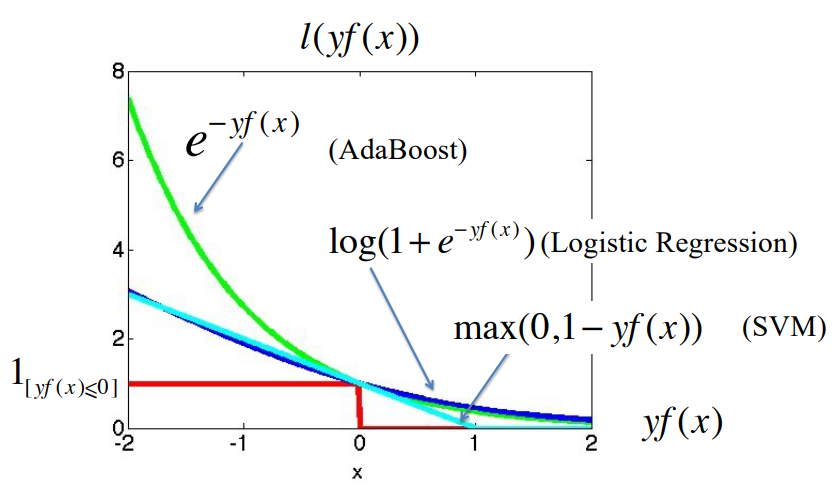
\includegraphics[scale=0.35]{img/loss_functions_class.png}
    \end{center}

    In the perceptron, we would want a function that penalizes not only if there is a misclassification, but how \textit{far} that misclassified point is from the boundary. Therefore, if $y^{(n)}$ and $h_\mathbf{w} (\mathbf{x}^{(n)})$ have the same sign, i.e. if $y^{(n)} h_\mathbf{w} (\boldsymbol{\phi}^{(n)}) > 0$, then the penalty should be $0$, and if it is $< 0$, then the penalty should be proportional to the orthogonal distance of the misclassified point to the boundary, which is represented by $-\mathbf{w}^T \boldsymbol{\phi}^{(n)} y^{(n)}$ (where the negative sign makes this cost term positive). To define our final cost function, let us define the function 
    \begin{equation}
      [f(\mathbf{x})]_+ \coloneqq \begin{cases} f(\mathbf{x}) & \text{ if } f(\mathbf{x}) > 0 \\ 0 & \text{ else } \end{cases}
    \end{equation}

    Therefore, our cost functions would take all the points and penalize all the terms by $0$ if they are correctly classified and by $-\mathbf{w}^T \boldsymbol{\phi}^{(n)} y^{(n)}$ if incorrectly classified. 
    \begin{equation}
      E(\mathbf{w}) = \sum_{n=1} [ -\mathbf{w}^T \boldsymbol{\phi}^{(n)} y^{(n)} ]_+
    \end{equation}
    which is a piecewise linear function and therefore can be optimized. In fact, it can be proven that if a dataset is \textbf{linearly separable}, i.e. if there exists an affine hyperplane separating the two classes, then the perceptron is guaranteed to find it. Therefore, the gradient descent algorithm
    \begin{equation}
      \mathbf{w}^{(\tau + 1)} = \mathbf{w}^{(\tau)} - \eta \nabla E(\mathbf{w})
    \end{equation}
    which is easier to interpret as SGD updating one partial at a time
    \begin{equation}
      \mathbf{w}^{(\tau + 1)} = \mathbf{w}^{(\tau)} - \eta \frac{\partial E(\mathbf{w})}{\partial w_n} \bigg|_{\mathbf{w}^{(\tau)}}
    \end{equation}
    where by abuse of notation, the partial represents the vector of $0$'s except for the $n$th term, will convergence to a solution if one exists. However, it does not guarantee that every step of GD will reduce the error. 

    Let's implement this in scikit-learn, using two pipelines with different data standardization techniques to see the differences in the perceptron boundary. 

    \begin{figure}[H]
      \centering 
      \begin{lstlisting}
        from sklearn.pipeline import Pipeline 
        from sklearn.linear_model import Perceptron
        from sklearn.preprocessing import QuantileTransformer, StandardScaler

        pipe1 = Pipeline([ 
            ("scale", StandardScaler()), 
            ("model", Perceptron())
        ])

        pipe2 = Pipeline([
            ("scale", QuantileTransformer(n_quantiles=100)), 
            ("model", Perceptron())
        ])
      \end{lstlisting}
      \caption{} 
      \label{fig:Perceptron_Code}
    \end{figure}

    \begin{figure}[H]
      \centering
      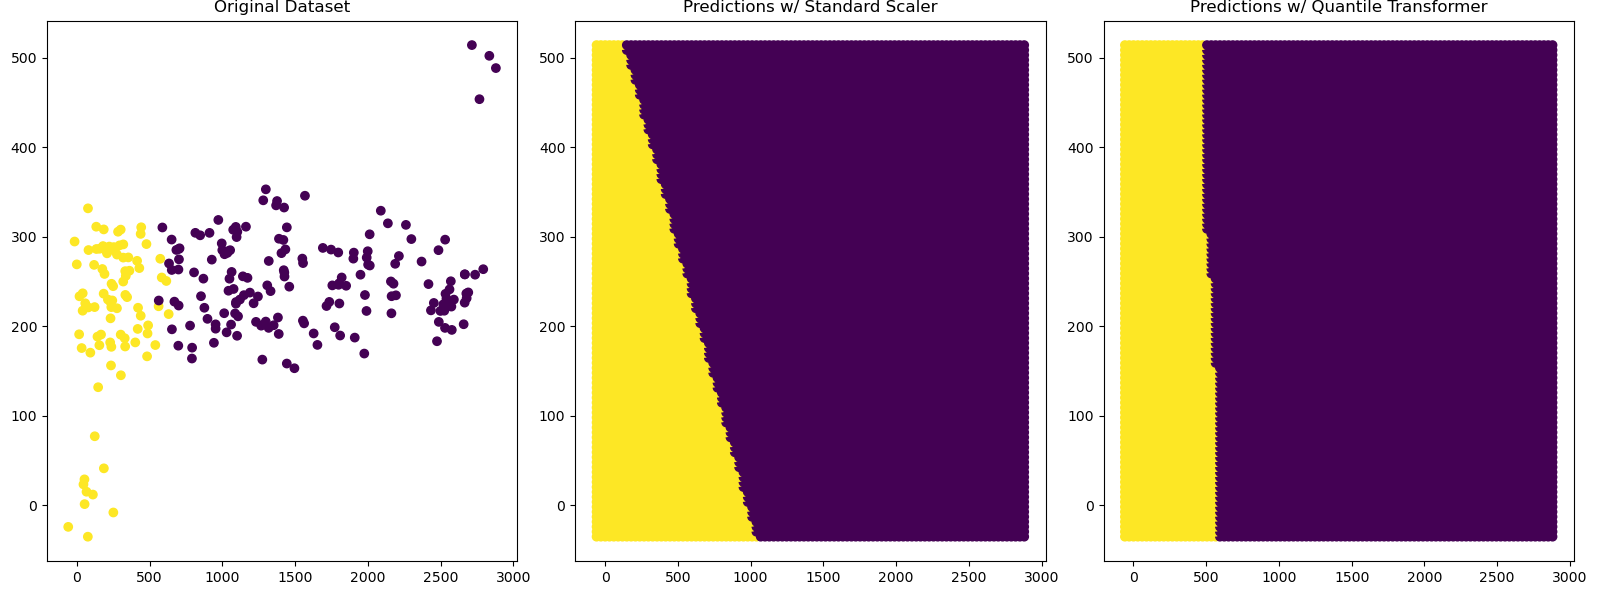
\includegraphics[scale=0.4]{img/Perceptron.png}
      \caption{Perceptron Trained on Different Standardized Data}
      \label{fig:Percepton_on_Standardized_data}
    \end{figure}


  \subsection{Logistic and Softmax Regression} 

    \subsubsection{Sparse Logistic Regression}

  \subsection{Support Vector Machines}

\section{Nonparametric Classification}

  \subsection{K Nearest Neighbors} 

    \begin{question}[To Do]
      Maybe similar like a kernel regression?  
    \end{question}

    Given a bunch of points in a metric space $(\mathcal{X}, d)$ that have classification labels, we want to label new datapoints $\hat{\mathbf{x}}$ based on the labels of other points that already exist in our dataset. One way to look at it is to look for close points within the dataset and use their labels to predict the new ones. 

    \begin{definition}[Closest Neighborhood]
      Given a dataset $\mathcal{D} = \{\mathbf{x}^{(i)}, \mathbf{y}^{(i)}\}$ and a point $\hat{\mathbf{x}} \in (\mathcal{X}, d)$, let the \textbf{k closest neighborhood} of $\hat{\mathbf{x}}$ be $N_k (\hat{\mathbf{x}}) \subset [N]$ defined as the indices $i$ of the $k$ points in $\mathcal{D}$ that is closest to $\hat{\mathbf{x}}$ with respect to the distance metric $d_\mathcal{X}$. 
    \end{definition}

    \begin{definition}[K Nearest Neighbors]
      The \textbf{K Nearest Neighbors (KNN)} is a discriminative nonparametric supervised learning algorithm that doesn't have a training phase. Given a new point $\hat{\mathbf{x}}$, we look at all points in its k closest neighborhood, and $h(\hat{\mathbf{x}})$ will be equal to whatever the majority class will be in. Let us one-hot encode the labels $\mathbf{y}^{(i)}$ into $\mathbf{e}_i$'s, and the number of data point in the $i$th class can be stored in the variable 
      \begin{equation}
        a_i = \sum_{i \in N_k (\hat{\mathbf{x}})} 1_{\{\mathbf{y}^{(i)} = \mathbf{e}_i\}}
      \end{equation}
      which results in the vector storing the counts of labels in the k closest neighborhood 
      \begin{equation}
        \mathbf{a} = (a_1, a_2, \ldots, a_\mathcal{K}) = \bigg( \sum_{i \in N_k (\hat{\mathbf{x}})} 1_{\{\mathbf{y}^{(i)} = \mathbf{e}_1\}}, \sum_{i \in N_k (\hat{\mathbf{x}})} 1_{\{\mathbf{y}^{(i)} = \mathbf{e}_2\}}, \ldots, \sum_{i \in N_k (\hat{\mathbf{x}})} 1_{\{\mathbf{y}^{(i)} = \mathbf{e}_\mathcal{K}\}} \bigg) 
      \end{equation}
      and take the class with the maximum element as our predicted label. 
    \end{definition}

    The best choice of $K$ depends on the data: 
    \begin{enumerate}
      \item Larger values of $K$ reduces the effect of noise on the classification, but make boundaries between classes less distinct. The number of misclassified data points (error) increases. 
      \item Smaller values are more sensitive to noise, but boundaries are more distinct and the number of misclassified data points (error) decreases.
    \end{enumerate}
    Too large of a $K$ value may increase the error too much and lead to less distinction in classification, while too small of a k value may result in us overclassifying the data. Finally, in binary (two class) classification problems, it is helpful to choose $K$ to be odd to avoid tied votes.

    This is an extremely simple algorithm that may not be robust. For example, consider $K \geq 3$, and we are trying to label a point $\hat{\mathbf{x}}$ that happens to be exactly where one point is on our dataset $\mathbf{x}^{(i)}$. Then, we should do $h(\hat{\mathbf{x}}) = y^{(i)}$, but this may not be the case if there are no other points with class $y^{(i)}$ in the k closest neighborhood of $\mathbf{x}^{(i)}$. Therefore, we want to take into account the distance of our new points from the others. 

    \begin{definition}[Weighted Nearest Neighbor Classifier]
      Let us define a monotinically decreasing function $\omega: \mathbb{R}_0^+ \mapsto \mathbb{R}_0^+$. Given a point $i \in N_k (\hat{\mathbf{x}})$, we can construct the weight of our matching label as inversely proportional to the distance: $\omega_i [ d(\hat{\mathbf{x}}, \mathbf{x}^{(i)})]$ and store them as 
      \begin{equation}
        \mathbf{a} = (a_1, a_2, \ldots, a_\mathcal{K}) = \bigg( \sum_{i \in N_k (\hat{\mathbf{x}})} \omega_i 1_{\{\mathbf{y}^{(i)} = \mathbf{e}_1\}}, \sum_{i \in N_k (\hat{\mathbf{x}})} \omega_i 1_{\{\mathbf{y}^{(i)} = \mathbf{e}_2\}}, \ldots, \sum_{i \in N_k (\hat{\mathbf{x}})} \omega_i 1_{\{\mathbf{y}^{(i)} = \mathbf{e}_\mathcal{K}\}} \bigg)
      \end{equation}
      and again take the class with the maximum element. 
    \end{definition}

    One caveat of KNN is in high dimensional spaces, as its performance degrades quite badly due to the curse of dimensionality. 

    \begin{example}[Curse of Dimensionality in KNN]
      Consider a dataset of $N$ samples uniformly distributed in a $d$-dimensional hypercube. Now given a point $x \in [0, 1]^d$, we want to derive the expected radius $r_k$ required to encompass its $k$ nearest neighbors. Let us define this ball to be $B_{r_k} \coloneqq \{ z \in \mathbb{R}^d \mid ||z - x ||_2 \leq r_k \}$. Since thse $N$ points are uniformly distributed, the expected number of points contained in $B_{r_k} (x)$ is simply the proportion of the volume that $B_{r_k} (x)$ encapsulates in the box, multiplied by $N$. Therefore, for some fixed $x$ and $r$, let us denote $Y(x, y)$ as the random variable representing the number of points contained within $B_r (x)$. By linearity of expectation and summing over the expectation for whether each point will be in the ball, we have 
      \[\mathbb{E}[Y (x, r)] = N \cdot \frac{\mu(B_r (x) \cap [0, 1]^d) }{\mu([0, 1]^d)}\]
      where $\mu$ is the Lebesgue measure of $\mathbb{R}^d$. Let us assume for not that we don't need to worry about cases where the ball is not fully contained within the cube, so we can just assume that $Y$ is only dependent on $r$: $Y(r)$. Also, since the volume of the hypercube is $1$,  $\mu([0, 1]^d) = 1$ and we get 
      \[\mathbb{E}[Y(r)] = N \cdot C_d \cdot r^d\]
      which we set equal to $k$ and evaluate for $r$. $C_d$ is a constant such that the volume of the hypersphere of radius $r$ can be derived as $V = C_d \cdot r^d$. We therefore get 
      \[N \cdot C_d \cdot r_k^d = k \implies r_k = \bigg( \frac{k}{N C_d} \bigg)^{1/d}\]
      It turns out that $C_d$ decreases exponentially, so the radius $r_k$ explodes as $d$ grows. Another way of looking at this is that in high dimensions, the $\ell_2$ distance between all the pairwise points are close in every single dimension, so it becomes harder to distinguish points that are close vs those that are far.  
    \end{example} 

  \subsection{Classification Trees}

    \begin{definition}[Decision Trees]
      Like K nearest neighbors, \textbf{decision trees} are discriminative nonparametric classification algorithms that involves creating some sort of tree that represents a set of decisions using a given set of input data $\mathbf{x}^{(i)}$ with its given classification $\mathbf{y}^{(i)}$. When predicting the class of a new input $\hat{\mathbf{x}}$, we would look at its attributes in some order, e.g. $\hat{x_1}, \hat{x}_2, \hat{x}_3$, and make a decision on which class it is in. 
      \begin{center}
          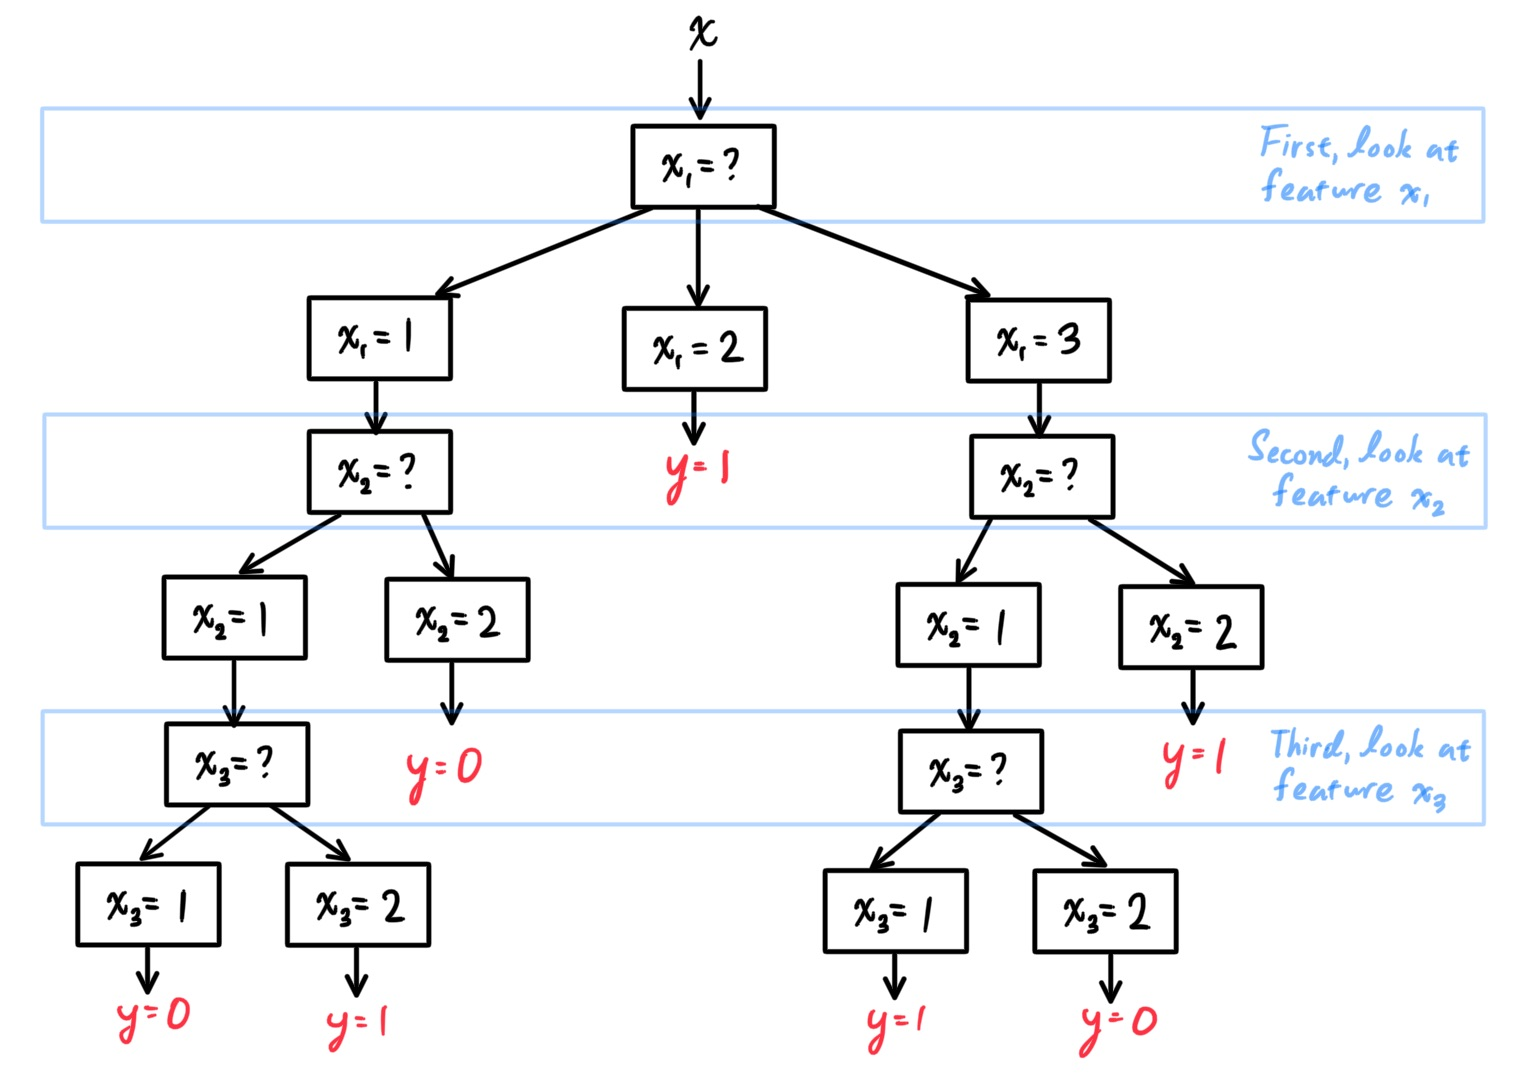
\includegraphics[scale=0.2]{img/general_decision_tree.jpg}
      \end{center}
      The decision tree tries to take advantage of some nontrivial covariance between $X$ and $Y$ by constructing nested partitions of the dataset $\mathcal{D}$, and within a partition, it predicts the label that comprises the majority. 
    \end{definition}

    For now, let us assume that $\mathcal{X}$ is a Cartesian product of discrete sets, and we will extend them to continuous values later. Let us look at an example to gain some intuition. 

    \begin{example}[Restaurant]
      Consider the dataset 
      \begin{center}
        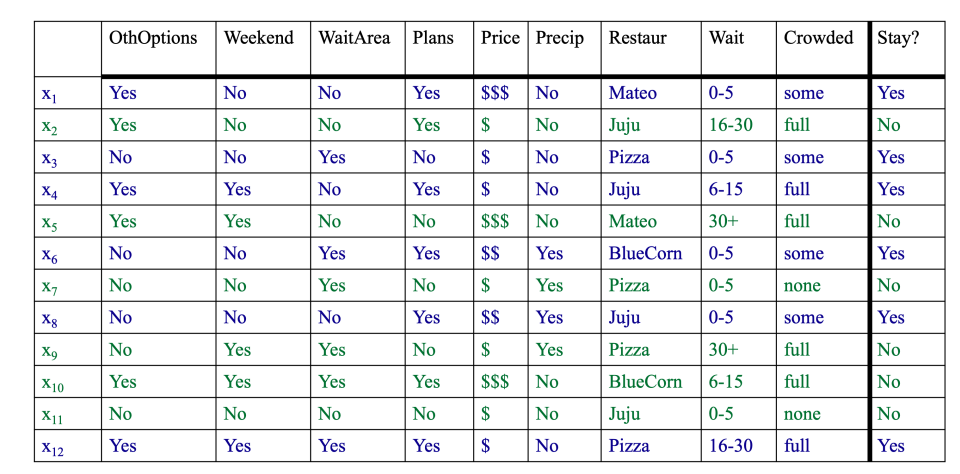
\includegraphics[scale=0.4]{img/decision_data.png}
      \end{center}
      Let us denote $\mathcal{D}$ as the dataset, and say that $F_1, \ldots, F_d$ were the features. This is a binary classification problem, and we can count that there are $6$ positives and $6$ negative labels. 
    \end{example}

    The simplest decision tree is the trivial tree, with one node that predicts the majority of the dataset. In this case, the data is evenly split, so without loss of generality we will choose $h_0 (\mathbf{x}) = 1$. We want to quantify how good our model is, and so like always we use a loss function. 

  \subsection{Splitting Criteria}

    Just like how a linear model is completely defined by its parameter $\boldsymbol{\theta}$, a decision tree is completely defined by the sequences of labels that it splits on. Therefore, training this is equivalent to defining the sequence, but we can't define this sequence unless we can compare how good a given decision tree is, i.e. unless we have defined a proper loss function. Depending on the training, we can use a greedy algorithm or not, and we have the flexibility to choose whether or not we can split on the same feature multiple times. 

    \subsubsection{Misclassification Error}

      \begin{definition}[Musclassification Error]
        We will simply use the misclassification loss function. 
        \begin{equation}
          L(h; \mathcal{D}) = \frac{1}{N} \sum_{i=1}^N 1_{\{y^{(i)} \neq h(x^{(i)})\}} = 1 - \text{accuracy}
        \end{equation}
        Minimizing this maximizes the accuracy, so this is a reasonable one to choose. How do we train this? Unlike regression, this loss is not continuous, so the gradient is $0$, and furthermore the model isn't even parametric, so there are no gradients to derive! 
      \end{definition}

      Fortunately, the nature of the decision tree only requires us to look through the explanatory variables $x_1, \ldots, x_n$ and decide which one to split. 

    \subsubsection{Information Gain}

      Let us take a decision tree $h$ and model the accuracy of it as a random variable: $1_{\{Y = h_0 (X)\}} \sim \mathrm{Bernoulli}(p)$, where $p$ is the accuracy. A higher accuracy of $h$ corresponds to a lower entropy, and so the entropy of the random variable is also a relevant indicator. 
      \[H(1_{\{Y = h_0 (X)\}}) = p \log{p} + (1 - p) \log(1 - p)\]
      Therefore, when we are building a tree, we want to choose the feature $x_i$ to split based on how much it lowers the entropy of the decision tree. 

      To set this up, let us take our dataset $\mathcal{D}$ and set $X_i$ as the random variable representing the distribution (a multinomial) of the $x_i^{(j)}$'s, and $Y$ as the same for the $y^{(j)}$'s. This is our maximum likelihood approximation for the marginalized distribution of the joint measure $X \times Y = X_1 \times \ldots \times X_D \times Y$. 

      Given a single node, we are simply going to label every point to be whatever the majority class is in $\mathcal{D}$. Therefore, we start off with the entropy of our trivial tree $H(Y)$. Then, we want to see which one of the $X_d$ features to split on, and so we can compute the conditional entropy $H(Y, X_d)$ to get the information gain $I(Y; X_d) = H(Y) - H(Y \mid X_d)$ for all $d = 1, \ldots, D$. We want to find a feature $X_d$ that maximize this information gain, i.e. decreases the entropy as much as possible (a greedy algorithm), and we find the next best feature (with or without replacement), so that we have a decreasing sequence. 
      \[H(X) \geq H(X ; Y) \geq H(X ; Y, Z) \geq H(X ; Y, Z, W) \geq \ldots \geq 0\]

      \begin{example}
      Continuing the example above, since there are $6$ labels of $0$ and $1$ each, we can model this $Y \sim \mathrm{Bernoulli}(0.5)$ random variable, with entropy 
      \[H(Y) = \mathbb{E}[-\log_2 p(Y)] = \frac{1}{2} \big( -\log_2 \frac{1}{2} \big) + \frac{1}{2} \big( -\log_2 \frac{1}{2} \big) = 1\]
      Now what would happen if we had branched according to how crowded it was, $X_{\mathrm{crowded}}$. Then, our decision tree would split into 3 sections: 
      \begin{center}
        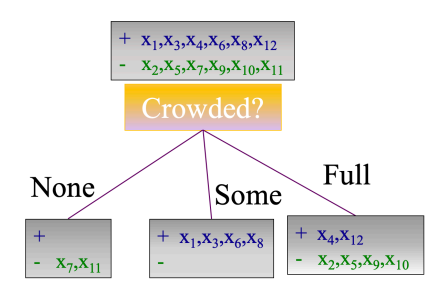
\includegraphics[scale=0.5]{img/decision_crowded.png}
      \end{center}
      In this case, we can define the multinomial distribution $X_{\mathrm{crowded}}$ representing the proportion of the data that is crowded in a specific level. That is, $X_{\mathrm{crowded}} \sim \mathrm{Multinomial}(\frac{2}{12}, \frac{4}{12}, \frac{6}{12} \big)$, with 
      \[\mathbb{P}(X_{\mathrm{crowded}} = x) = \begin{cases} 2/12 & \text{ if } x = \text{ none} \\ 4/12 & \text{ if } x = \text{ some} \\ 6/12 & \text{ if } x = \text{ full} \end{cases} \]
      Therefore, we can now compute the conditional entropy of this new decision tree conditioned on how crowded the store is 
      \begin{align*}
          H(Y \mid X_{\mathrm{crowded}}) & = \sum_x \mathbb{P}(X_{\mathrm{crowded}} = x) H(Y \mid X_{\mathrm{crowded}} = x) \\
          & = \frac{2}{12} H(\mathrm{Bern}(1)) + \frac{4}{12} H(\mathrm{Bern}(0)) + \frac{6}{12} H(\mathrm{Bern}(1/3)) = 0.459 \\
          I(Y; X_{\mathrm{crowded}}) & = 0.541
      \end{align*}
      We would do this for all the features and greedily choose the feature that maximizes our information gain. 
      \end{example}

      \begin{example}
      The Ferrari F1 team hired you as a new analyst! You were given the following table of the past race history of the team. You were asked to use information gain to build a decision tree to predict race wins. First, you will need to figure out which feature to split first. 

      \begin{center}
      \begin{tabular}[c]{c|c|c||c}
      Rain & Good Strategy & Qualifying & Win Race \\ \hline
      1 & 0 & 0 & 0 \\
      1 & 0 & 0 & 0 \\
      1 & 0 & 1 & 0 \\
      0 & 0 & 1 & 1 \\
      0 & 0 & 0 & 0 \\
      0 & 1 & 1 & 1 \\
      1 & 0 & 1 & 0 \\
      0 & 1 & 0 & 1 \\
      0 & 0 & 1 & 1 \\
      0 & 0 & 1 & 1 \\
      \end{tabular}
      \end{center}
      Let $X \sim \mathrm{Bernoulli}(1/2)$ be the distribution of whether a car wins a race over the data. Then its entropy is 
      \[H(X) = \mathbb{E}[-\log_2 p(x)] = \frac{1}{2} \big( -\log_2 \frac{1}{2} \big) + \frac{1}{2} \big( -\log_2 \frac{1}{2} \big) = 1\]
      Let $R \sim \mathrm{Bernoulli}(4/10), G \sim \mathrm{Bernoulli}(2/10), Q \sim \mathrm{Bernoulli}(6/10)$ be the distribution of the features rain, good strategy, and qualifying over the data, respectively. Then, the conditional entropy of $X$ conditioned on each of these random variables is 
      \begin{align*}
          H(X \mid R) & = \mathbb{P}(R = 1)\, H(X \mid R = 1) + \mathbb{P}(R = 0) \, H(X \mid R = 0) \\
          & = \frac{4}{10} \cdot - \big( 1 \cdot \log_2 1 + 0 \cdot \log_2 0 \big) + \frac{6}{10} \cdot - \big( \frac{1}{6} \cdot \log_2 \frac{1}{6} + \frac{5}{6} \cdot \log_2 \frac{5}{6} \big) \approx 0.390 \\
          H(X \mid G) & =  \mathbb{P}(G = 1)\, H(X \mid G = 1) + \mathbb{P}(G = 0) \, H(X \mid G = 0) \\
          & = \frac{2}{10} \cdot - \big( 1 \cdot \log_2 1 + 0 \cdot \log_2 0 \big) + \frac{8}{10} \cdot - \big( \frac{3}{8} \cdot \log_2 \frac{3}{8} + \frac{5}{8} \log_2 \frac{5}{8} \big) \approx 0.763\\
          H(X \mid Q ) & = \mathbb{P}(Q = 1)\, H(X \mid Q = 1) + \mathbb{P}(Q = 0) \, H(X \mid Q = 0) \\
          & = \frac{6}{10} \cdot - \big( \frac{4}{6} \cdot \log_2 \frac{4}{6} + \frac{2}{6} \cdot \log_2 \frac{2}{6} \big) + \frac{4}{10} \cdot - \big( \frac{1}{4} \log_2 \frac{1}{4} + \frac{3}{4} \log_2 \frac{3}{4} \big) \approx 0.875
      \end{align*}
      Therefore, the information gain are 
      \begin{align*}
          I(X; R) & = 1 - 0.390 = 0.610 \\
          I(X; G) & = 1 - 0.763 = 0.237 \\
          I(X; Q) & = 1 - 0.875 = 0.125 
      \end{align*}
      And so I would split on $R$, the rain, which gives the biggest information gain. 
      \end{example}

    \subsubsection{Gini Index}

      Finally, we can use the Gini index of $X \sim \mathrm{Bernoulli}(p)$, defined 
      \begin{equation}
        G(X) = 2 p (1 - p)
      \end{equation}

      \begin{example}[Ferrari Example Continued]
        We do the same as the Ferrari example above but now with the Gini reduction. Let $X \sim \mathrm{Bernoulli}(1/2)$ be the distribution of whether a car wins a race over the data. Then its Gini index, which I will label with $\mathcal{G}$, is \[\mathcal{G} (X) = 2 \cdot \frac{1}{2} \cdot \frac{1}{2} = \frac{1}{2}\]
        Let $R \sim \mathrm{Bernoulli}(4/10), G \sim \mathrm{Bernoulli}(2/10), Q \sim \mathrm{Bernoulli}(6/10)$ be the distribution of the features rain, good strategy, and qualifying over the data, respectively. Then we compute the conditional expectation 
        \begin{align*}
            \mathbb{E}[\mathcal{G}(X \mid R)] & = \mathbb{P}(R = 1)\, \mathcal{G}(X \mid R = 1) + \mathbb{P}(R = 0) \, \mathcal{G}(X \mid R = 0) \\ 
            & = \frac{4}{10} \bigg[ 2 \cdot \frac{4}{4} \cdot \frac{0}{4} \bigg] + \frac{6}{10} \bigg[ 2 \cdot \frac{1}{6} \cdot \frac{5}{6} \bigg] \approx 0.167 \\
            \mathbb{E}[\mathcal{G}(X \mid G)] & = \mathbb{P}(G = 1)\, \mathcal{G}(X \mid G = 1) + \mathbb{P}(G = 0) \, \mathcal{G}(X \mid G = 0) \\ 
            & = \frac{2}{10} \bigg[ 2 \cdot \frac{2}{2} \cdot \frac{0}{2} \bigg] + \frac{8}{10} \bigg[ 2 \cdot \frac{3}{8} \cdot \frac{5}{8} \bigg] \approx 0.375 \\
            \mathbb{E}[\mathcal{G}(X \mid Q)] & = \mathbb{P}(Q = 1)\, \mathcal{G}(X \mid Q = 1) + \mathbb{P}(Q = 0) \, \mathcal{G}(X \mid Q = 0) \\ 
            & = \frac{6}{10} \bigg[ 2 \cdot \frac{4}{6} \cdot \frac{2}{6} \bigg] + \frac{4}{10} \bigg[ 2 \cdot \frac{1}{4} \cdot \frac{3}{4} \bigg] \approx 0.417
        \end{align*}
        Therefore, the Gini reduction, which I'll denote as $I_{\mathcal{G}}$, is 
        \begin{align*}
            I_{\mathcal{G}} (X ; R) & = 0.5 - 0.167 = 0.333 \\
            I_{\mathcal{G}} (X ; G) & = 0.5 - 0.375 = 0.125 \\
            I_{\mathcal{G}} (X ; Q) & = 0.5 - 0.417 = 0.083
        \end{align*}
        Since branching across the feature $R$, the rain, gives the biggest Gini reduction, we want to split on the rain feature first. 
      \end{example}


    \subsection{Regularization}

    Given a dataset with $D$ binary features, let $g(H, D)$ be the number of binary trees with depth at most $H$ (including root node), with the restriction that the trees may not split on some variable multiple times within a path to a leaf node. Then, $g$ can be defined recursively. 
    \begin{enumerate}
        \item First, if $H = 1$, then $g(H, D) = 1$ always since we are just creating the trivial binary tree of one node. 
        \item If $D = 0$, then there are no features to split on and therefore we just have the single node $g(H, D) = 1$. 
        \item If $H > 1$ and $D > 0$, then say that we start with a node. We can either make this a leaf node by not performing any splitting at all, or split on one of the $D$ variables. Then for each of the 2 nodes created on the split, we are now working with $D-1$ features and a maximum height of $H-1$ for each of the subtrees generated from the 2 nodes. 
    \end{enumerate}
    All this can be expressed as 
    \[g(H, D) = \begin{cases} 1 + D \, \big[ g(H - 1, D - 1) \big]^2 & \text{ if } H > 1, D > 0 \\ 1 & \text{ if } H = 1 \text{ or } D = 0 \end{cases} \]
    which is extremely large (in fact, NP hard). Therefore, some tricks like regularization must be implemented to limit our search space. 

    By defining the complexity of our decision tree $\Omega(h)$ as the number of nodes within the tree, we can modify our objective function to 
    \[L(h; \mathcal{D}) = \frac{1}{N} \sum_{i=1}^N 1_{\{y^{(i)} \neq h(x^{(i)})\}} + \lambda \Omega(h)\]
    We can impose this constraint directly on the training algorithm, or we can calculate the regularized loss after the tree has been constructed, which is a method called \textbf{tree pruning}. 

    Given a large enough $\lambda$, we can in fact greatly reduce our search space by not considering any trees further than a certain point. 

    \begin{theorem}
    We describe a tree as a set of leaves, where leaf $k$ is a tuple containing the logical preposition satisfied by the path to leaf $k$, denoted $p_k $, and the class label predicted by the leaf, denoted $\hat{y}_k$. For a dataset with $d$ binary features, $p_k: \{0, 1\}^d \to \{0, 1\}$ is a function that returns $1$ if a sample $x_i$ satisfies the preposition, and $0$ otherwise. That is, leaf $k$ is $(p_k, \hat{y}_k),$ and a tree $f$ with $K$ leaves is described as a set $f = \{(p_1, \hat{y}_1), \hdots, (p_K, \hat{y}_K)\}$. Assume that the label predicted by $\hat{y}_k$ is always the label for the majority of samples satisfying $p_k$. Finally, let $m_k = \sum_{i=1}^n p_k(x_i)$ denote the number of training samples ``captured'' by leaf $k$.

    Given a (potentially optimal) tree 

      \[f = \{(p_1, \hat{y}_1), \hdots, (p_{\kappa}, \hat{y}_{\kappa}), \hdots, (p_K, \hat{y}_K)\}, \]

    the tree $f' = \{(p_1, \hat{y}_1), \hdots, (p_{\kappa_1}, \hat{y}_{\kappa_1}), (p_{\kappa_2}, \hat{y}_{\kappa_2}), \hdots, (p_K, \hat{y}_K)\}$ produced by splitting leaf $(p_{\kappa}, \hat{y}_{\kappa})$ into two leaves $(p_{\kappa_1}, \hat{y}_{\kappa_1})$ and $(p_{\kappa_2}, \hat{y}_{\kappa_2})$ and any tree produced by further splitting $(p_{\kappa_1}, \hat{y}_{\kappa_1})$ or $(p_{\kappa_2}, \hat{y}_{\kappa_2})$ cannot  be optimal if $m_{\kappa} < 2n\lambda$.
    \end{theorem}
    \begin{proof}
    Let $c$ be the number of misclassifications in leaf $(p_{\kappa}, \hat{y}_{\kappa})$. Since a leaf classifies according to the majority of $m_{\kappa}$, we must have 

      \[c \leq \frac{m_\kappa}{2} < n \lambda\]

    By splitting leaf $(p_\kappa, \hat{y}_\kappa)$ into leaves $(p_{\kappa_1}, \hat{y}_{\kappa_1})$ and $(p_{\kappa_2}, \hat{y}_{\kappa_2})$, assume that we have reduced the number of misclassifications by $b \leq c$. Then, we have 

      \[\ell(f^\prime, \mathbf{X}, \mathbf{y}) = \ell(f, \mathbf{X}, \mathbf{y}) - \frac{b}{n}\]

    However, we have increased the number of leaves by $1$, and so 

      \[\lambda s(f^\prime) = \lambda s(f) + \lambda\]

    Combining the last two equations, we have obtained 

      \[R (f^\prime, \mathbf{X}, \mathbf{y}) = R(f, \mathbf{X}, \mathbf{y}) + \lambda - \frac{b}{n}\]

    However, we know that 

    \begin{align*}
      b \leq c & \implies \frac{b}{n} \leq \frac{c}{n} < \frac{n \lambda}{n} = \lambda \\
      & \implies - \frac{b}{n} > - \lambda \\
      & \implies \lambda - \frac{b}{n} > \lambda - \lambda = 0
    \end{align*}

    and so $R (f^\prime, \mathbf{X}, \mathbf{y}) > R(f, \mathbf{X}, \mathbf{y})$. This means that $f^\prime$ cannot be optimal according to our regularized objective. We have also proved that further splitting $(p_{\kappa_1}, \hat{y}_{\kappa_1})$ or $(p_{\kappa_2}, \hat{y}_{\kappa_2})$ cannot  be optimal since we can just set $f = f^\prime$, and apply the same argument. 
    \end{proof}

\section{Generalized Linear Models} 

  Remember the linear model looked like this, where we use the conventional $\beta$ notation to represent parameters. 
  \begin{equation}
    Y = X^T \beta + \epsilon, \;\; \epsilon \sim N(0, \sigma^2 I)
  \end{equation}
  which implies that $Y \mid X \sim N(X^T \beta, \sigma^2 I)$. Basically, given $x$, I assume some distribution of $Y$, and the value of $x$ will help me guess what the mean of this distribution is. Note that we in here assume that only the mean depends on $X$. I could potentially have something crazy, like 
  \[Y \mid X \sim N(X^T \beta, (X^T \gamma) (X X^T + I))\]
  where the covariance will depend on $X$, too, but in this case we only assume that that mean is dependent on $X$. 
  \[Y \mid X \sim N(\mu(X), \sigma^2 I)\]
  where in the linear model, $\mu(X) = X^T \beta$. So, there are three assumptions we are making here: 
  \begin{enumerate}
    \item $Y \mid X$ is Gaussian. 
    \item $X$ only affects the mean of $Y \mid X$, written $\mathbb{E}[Y \mid X] = \mu(X)$. 
    \item $X$ affects the mean in a linear way, such that $\mu(X) = X^T \beta$. 
  \end{enumerate}
  So the two things we are trying to relax are: 
  \begin{enumerate}
    \item \textbf{Random Component}: the response variable $Y \mid X$ is continuous and normally distributed with mean $\mu = \mu(X) = \mathbb{E}[Y \mid X]$. 
    \item \textbf{Link}: I have a link that explains the relationship between the $X$ and the $\mu$, and this relationship is $\mu(X) = X^T \beta$. 
  \end{enumerate}
  So when talking about GLMs, we are not changing the fact that we have a linear function $X \mapsto X^T \beta$. However, we are going to assume that $Y \mid X$ now comes from a broader \textbf{family of exponential distributions}. Second, we are going to assume that there exists some \textbf{link function} $g$
  \[g(\mu(X)) = X^T \beta\]
  Admittedly, this is not the most intuitive way to think about it, since we would like to have $\mu(X) = f(X^T \beta)$, but here we just decide to call $f = g^{-1}$. Therefore, if I want to give you a GLM, I just need to give you two things: the conditional distribution $Y \mid X$, which can be any distribution in the exponential family, and the link function $g$. 

  We really only need this link function due to compatibility reasons. Say that $Y \mid X \sim \mathrm{Bern}(p)$. Then, $\mu(X) = \mathbb{E}[Y \mid X]$ always lives in $[0, 1]$, but $X^T \beta$ always lives in $\mathbb{R}$. We want our model to be realistic, and we can clearly see the problem shown in Figure \ref{fig:Bernoulli_GLM}. 

  \begin{figure}[H]
    \centering
    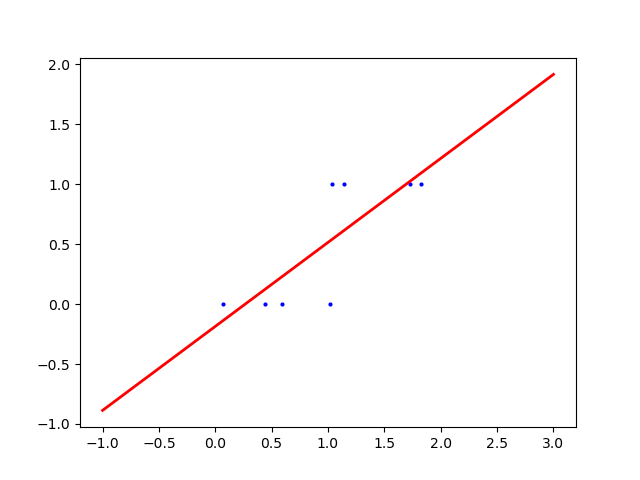
\includegraphics[scale=0.5]{img/GLM_bernoulli.png}
    \caption{Fitting a linear model for Bernoulli random variables will predict a mean that is outside of $[0, 1]$ when getting new datapoints. }
    \label{fig:Bernoulli_GLM}
  \end{figure}

  If $Y \mid X$ is some exponential distribution, then its support is always positive and so $\mu(X) > 0$. But if we stick to the old form of $\mu(X) = X^T \beta$, then $\mathrm{Im}(\mu) = \mathbb{R}$, which is not realistic when we predict negative values. Let's take a couple examples: 

  \begin{example}[Disease Epidemic]
    In the early stages of a disease epidemic, the rate at which new cases occur can often increase exponentially through time. Clearly, $\mu(X) = \mathbb{E}[Y \mid X]$ should be positive and we should have some sort of exponential trend. Hence, if $\mu(x)$ is the expected number of cases on data $x$, a model of the form 
    \begin{equation}
      \mu(x) = \gamma \exp (\delta x)
    \end{equation}
    seems appropriate, where $\gamma$ and $\delta$ are simply scaling factors. Clearly, $\mu(X)$ is not of the form $f(X^T \beta)$. So what I do is to transform $\mu$ in such a way that I can get something that is linear. 
    \begin{equation}
      \log(\mu(X)) = \log(\gamma) + \delta X
    \end{equation}
    which is now linear in $X$, of form $\beta_0 + \beta_1 X$. This will have some effects, but this is what needs to be done to have a genearlized linear model. Note that what I did to $\mu$ was take the log of it, and so the link function is $g = \log$, called the \textbf{log-link}. Now that we have chosen the $g$, we still need to choose what the conditional distribution $Y \mid X$ would be. This is determined by speaking with industry professionals, experience, and convenience. In this case, $Y$ is a count, and since this must be a discrete distribution. Since it is not bounded above, we think Poisson. 
  \end{example}

  \begin{example}[Prey Capture Rate]
    The rate of capture of preys, $Y$, by a hunting animal, tends to increase with increasing density of prey $X$, but eventually level off when the predator is catching as much as it can cope with. We want to find a perhaps concave function that levels off, and suitable model might be 
    \begin{equation}
      \mu(X) = \frac{\alpha X}{h + X}
    \end{equation}
    where $\alpha$ represents the maximum capture rate, and $h$ represents the prey density at which the capture rate is half the maximum rate. Again, we must find some transformation $g$ that turns this into a linear function of $X$, and what we can do it use the \textbf{reciprocal-link}. 
    \begin{equation}
      \frac{1}{\mu(X)} = \frac{h + X}{\alpha X} = \frac{h}{\alpha} \frac{1}{X} + \frac{1}{\alpha}
    \end{equation}
    The standard deviation of capture rate might be approximately proportional to the mean rate, suggesting the use of a Gamma distribution for the response. 
  \end{example}

  \begin{example}[Kyphosis Data]
    The Kyphosis data consist of measurements on $81$ children following corrective spinal surgery. The binary response variable, Kyphosis, indicates the presence or absence of a postoperative deforming. The three covariates are: age of the child in months, number of the vertebrae involved in the operation, and the start of the range of the vertebrae involved. The response variable is binary so there is no choice: $Y \mid X$ is Bernoulli with expected value $\mu(X) \in (0, 1)$. We cannot write $\mu(X) = X^T \beta$ because the right hand side ranges through $\mathbb{R}$, and so we find an invertible function that squishes $\mathbb{R}$ to $(0, 1)$, and so we can choose basically any CDF. 
  \end{example}

  For clarification, when writing a distribution like $\mathrm{Bernoulli}(p)$, or $\mathrm{Binomial}(n, p)$, $\mathrm{Poisson}(\lambda)$, or $N(\mu, \sigma^2)$, the hyperparameters that we usually work with we will denote as $\boldsymbol{\theta}$, and the space that this $\boldsymbol{\theta}$ lives in will denote $\Theta$. For example, for the Bernoulli, $\Theta = [0, 1]$, and for Poisson, $\Theta = [0, +\infty)$. 

  Ultimately, a GLM consists of three steps: 
  \begin{enumerate}
    \item The observed input $X$ enters the model through a linear function $\beta^T X$. 
    \item The conditional mean of response, is represented as a function of the linear combination 
      \begin{equation}
        \mathbb{E}[Y \mid X] = \mu = f(\beta^T X)
      \end{equation}
    \item The observed response is drawn from an exponential family distribution with conditional mean $\mu$. 
  \end{enumerate}

  \subsection{Exponential Family}

    We can write the pdf of a distribution as a function of the input $x$ and the hyperparameters $\theta$, so we can write $P_\theta (x) = p(\theta, x)$. For now, let's think that both $x, \theta \in \mathbb{R}$. Think of all the functions that depend on $\theta$ and $x$. There are many of them, but we want $\theta$ and $x$ to interact in a certain way. The way that I want them to interact with each other is that they are multiplied within an exponential term. Now clearly, this is not a very rich family, so we are just slapping some terms that depend only on $\theta$ and only on $x$. 
    \[p_\theta (x) = \exp(\theta x) h(x) c(\theta)\]
    But now if $\theta \in \mathbb{R}^k$ and $x \in \mathbb{R}^q$, then we cannot simply take the product nor the inner product, but what we can do is map both of them into a space that has the same dimensions, so I can take the inner product. That is, let us map $\boldsymbol{\theta} \mapsto \boldsymbol{\eta}(\boldsymbol{\theta}) \in \mathbb{R}^k$ and $\mathbf{x} \mapsto \mathbf{T}(\mathbf{x}) \in \mathbb{R}^k$, and so 
    our exponential distribution form would be generalized into something like 
    \[p_{\boldsymbol{\theta}} (\mathbf{x}) = \exp\big[ \boldsymbol{\eta}(\boldsymbol{\theta}) \cdot \mathbf{T}(\mathbf{x}) \big] h(\mathbf{x}) c(\boldsymbol{\theta})\]
    We can think of $c(\boldsymbol{\theta})$ as the normalizing term that allows us to integrate the pdf to $1$. 
    \[\int_\mathcal{X} p_{\boldsymbol{\theta}} (\mathbf{x}) = c(\boldsymbol{\theta}) \int \exp\big[\boldsymbol{\eta}(\boldsymbol{\theta}) \cdot \mathbf{T}(\mathbf{x}) \big] h(\mathbf{x})  \,d\mathbf{x}\]
    We can just push the $c(\boldsymbol{\theta})$ term into the exponential by letting $c(\boldsymbol{\theta}) = e^{-\log(c(\boldsymbol{\theta}))^{-1}}$ to get our definition. 

    \begin{definition}[Exponential Family]
      A \textbf{k-parameter exponential family} is a family of distributions with pdf/pmf of the form 
      \[p_{\boldsymbol{\theta}} (\mathbf{x}) = \exp\big[ \boldsymbol{\eta}(\boldsymbol{\theta}) \cdot \mathbf{T}(\mathbf{x}) - B(\boldsymbol{\theta}) \big] h(\mathbf{x})\]
      The $h$ term, as we will see, will not matter in our maximum likelihood estimation, so we keep it outside the exponential. 
      \begin{enumerate}
        \item $\boldsymbol{\eta}$ is called the \textbf{canonical parameter}. Given a distribution parameterized by the regular hyperparameters $\boldsymbol{\theta}$, we would like to parameterize it in a different way $\boldsymbol{\eta}$ under the function $\boldsymbol{\eta}: \Theta \rightarrow \mathbb{R}$
        \item $\mathbf{T}(\mathbf{x})$ is called the \textbf{sufficient statistic}. 
        \item $h(\mathbf{x})$ is a nonnegative scalar function. 
        \item $B(\boldsymbol{\theta})$ is the normalizing factor. 
      \end{enumerate}
    \end{definition}

    Let's look at some examples. 

    \begin{example}[Gaussian]
      If we put the coefficient into the exponential and expand the square term, we get 
      \[p_\theta (x) = \exp \bigg( \frac{\mu}{\sigma^2} \cdot x - \frac{1}{2\sigma^2} \cdot x^2 - \frac{\mu^2}{2 \sigma^2} - \log ( \sigma \sqrt{2 \pi}) \bigg)\] 
      where 
      \[\boldsymbol{\eta}(\boldsymbol{\theta}) = \begin{pmatrix} \mu /\sigma^2 \\ -1 / 2 \sigma^2 \end{pmatrix}, \; T(x) = \begin{pmatrix} x \\ x^2 \end{pmatrix}, \; B(\theta) = \frac{\mu^2}{2 \sigma^2} + \log(\sigma \sqrt{2 \pi}), \; h(x) = 1\]
      This is not a unique representation since we can take the $\log(\sqrt{2 \pi})$ out of the exponential, but why bother to do this when we can just stuff everything into $B$ and keep $h$ simple. 
    \end{example}

    \begin{example}[Gaussian with Known Variance]
      If we have known variance, we can write the Gaussian pdf as 
      \[p_\theta (x) = \exp \bigg[ \frac{\mu}{\sigma} \cdot \frac{x}{\sigma} - \frac{\mu^2}{2 \sigma^2} \bigg] \cdot \frac{1}{\sigma \sqrt{2\pi}} e^{x^2/2 \sigma^2}\]
      where 
      \[\eta(\theta) = \frac{\mu}{\sigma}, \; T(x) = \frac{x}{\sigma}, \; B(\theta) = \frac{\mu^2}{2 \sigma^2}, \; h(x) = \frac{1}{\sigma \sqrt{2 \pi}} e^{x^2/2 \sigma^2}\]
    \end{example}

    \begin{example}[Bernoulli]
    The pmf of a Bernoulli with $\theta$ is 
    \begin{align*}
        p_\theta (x) & = \theta^x (1 - \theta)^{(1 - x)} \\
        & = \exp \big[x \log (\theta) + (1 - x)\log(1 - \theta) \big] \\
        & = \exp \bigg( x \log \Big[ \frac{\theta}{1 - \theta} \Big] - \log \Big[ \frac{1}{1 - \theta} \Big] \bigg)
    \end{align*}
    where 
    \[\eta(\theta) = \log \Big[ \frac{\theta}{1 - \theta} \Big], \; T(x) = x, \; B(\theta) = \log \Big[ \frac{1}{1 - \theta} \Big], \; h(x) = 1\]
    \end{example}


    \begin{example}[Binomial with Known Number of Trials]
    We can transform a binomial with known $N$ as 
    \begin{align*}
      p_\theta (x) &  = \binom{N}{x} \theta^x  (1 - \theta)^{1 - x} \\
                   & = \exp \bigg[ x \ln \big( \frac{\theta}{1 - \theta} \Big) + \ln(1 - \theta) \bigg] \cdot \binom{N}{x} 
    \end{align*}
    where 
      \[\eta (\theta) = \ln \big( \frac{\theta}{1 - \theta} \Big), \; T(x) = x, \; B(\theta) = \ln(1 - \theta), \; h(x) = \binom{N}{x}\]
    \end{example}

    \begin{example}[Poisson]
    The pmf of Poisson with $\theta$ can be expanded 
    \begin{align*}
        p_\theta & = \frac{\theta^{-x}}{x!} e^{-\theta} \\
        & = \exp \big[ -\theta + x\log(\theta) - \log(x!) \big] \\
        & = \exp \big[ x \log(\theta) - \theta \big] \, \frac{1}{x!}
    \end{align*}
    where 
    \[\eta(\theta) = \log(\theta), \; T(x) = x, \; B(\theta) = \theta, \; h(x) = \frac{1}{x!}\]
    \end{example}

    However, the uniform is not in here. In fact, any distribution that has a support that does not depend on the parameter is not an exponential distribution. 

    Let us now focus on one parameter families where $\theta \in \Theta \subset \mathbb{R}$, which do not include the Gaussian (with unknown mean and variance, Gamma, multinomial, etc.), which has a pdf written in the form 
    \[p_\theta (x) = \exp \big[ \eta (\theta) \, T(x) - B(\theta) \big] \, h(x)\]


    \subsubsection{Canonical Exponential Family}

      Now a common strategy in statistical analysis is to reparamaterize a probability distribution. Suppose a family of probability distributions $\{P_\theta\}$ is parameterized by $\theta \in \Theta \subset \mathbb{R}$. If we have an invertible function $\eta: \Theta \rightarrow \mathcal{T} \subset \mathbb{R}$, then we can paramaterize the same family with $\eta$ rather than $\theta$, with no loss of information. Typically, it is the case that $\eta$ is invertible for exponential families, so we can just reparameterize the whole pdf and write 
      \[p_\eta (x) = \exp \big[ \eta \, T(x) - \phi(\eta) \big] \, h(x)\]
      where $\phi = B \circ \eta^{-1}$. 

      \begin{definition}[Canonical One-Parameter Exponential Family]
      A family of distributions is said to be in \textbf{canonical one-parameter exponential family} if its density is of form 
      \[p_\eta (x) = \exp \big[ \eta \, T(x) - \phi(\eta) \big] \, h(x)\]
      which is a subfamily of the exponential family. The function $\psi$ is called the \textbf{cumulant generating function}. 
      \end{definition}

      Before we move on, let us just provide a few examples. 

      \begin{example}[Poisson]
      The Poisson can be represented as 
      \[p_\theta (x) = \exp \big[ x \log{\theta} - \theta \big] \, \frac{1}{x!}\]
      Now let $\eta = \log{\theta} \implies \theta = e^{\eta}$. So, we can reparamaterize the density as 
      \[p_\eta(x) = \exp \big[ x \eta - e^\eta \big] \, \frac{1}{x!}\]
      where $P_\eta = \mathrm{Poisson}(e^\eta)$ for $\eta \in \mathcal{T} = \mathbb{R}$, compared to $P_\theta = \mathrm{Poisson}(\theta)$ for $\theta \in \Theta = \mathbb{R}^+$. 
      \end{example}

      \begin{example}[Gaussian]
      Recall that the Gaussian with known parameter $\sigma^2$ and unknown $\theta = \mu$ is in the exponential family, since we can expand it as 
      \[p_\theta (x) = \exp \bigg[ \frac{\mu}{\sigma^2} \cdot x - \frac{\mu^2}{2 \sigma^2} \bigg] \cdot \frac{1}{\sigma \sqrt{2\pi}} e^{x^2/2 \sigma^2}\]
      We can perform the change of parameter $\eta = \mu^2 / 2\sigma^2 \implies \mu = \sigma^2 \eta$, and substituting this in will give the canonical representation 
      \[p_\eta (x) = \exp \Big[ \eta x - \frac{\sigma^2 \eta^2}{2} \Big] \cdot \frac{1}{\sigma \sqrt{2\pi}} e^{x^2/2 \sigma^2}\]
      where now $P_\eta = N(\sigma^2 \eta, \sigma^2)$ for $\eta \in \mathcal{T} = \mathbb{R}$, compared to $P_\theta = N(\theta, \sigma^2)$ for $\theta \in \Theta = \mathbb{R}$, which is basically the same space. 
      \end{example}

      \begin{example}[Bernoulli]
      The Bernoulli has an exponential form of 
      \[p_\theta (x) = \exp \bigg[ x \log \Big( \frac{\theta}{1 - \theta} \Big) + \log(1 - \theta)\bigg]\]
      Now setting $\eta = \log\big( \frac{\theta}{1 - \theta} \big) \implies \theta = \frac{1}{1 + e^{-\eta}}$, and so $B(\theta) = - \log(1 - \theta) = - \log \big( \frac{e^{-\eta}}{1 + e^{-\eta}} \big) = \log(1 + e^\eta) = \psi(\eta)$, and so the canonical paramaterization is 
      \[p_\eta (x) = \exp \big[ x \eta - \log(1 + e^{\eta}) \big]\]
      \end{example}


      We present two useful properties of the exponential family. 

      \begin{theorem}[Moments]
      Let random variable $X$ be in the canonical exponential family $P_\eta$ 
      \[p_\eta (x) = e^{\eta T(x) - \psi(\eta)} h(x)\]
      Then, the expectation and variance are encoded in the cumulant generating function in the following way 
      \[\mathbb{E} [T(X)] = \psi^\prime (\eta) \;\;\;\;\;\;\;\; \Var[T(X)] = \psi^{\prime\prime} (\eta)\]
      \end{theorem}
      \begin{proof}

      \end{proof}

      \begin{example}
      We show that this is consistent with the Poisson, normal, and Bernoulli distributions. 
      \begin{enumerate}
          \item In the Poisson, $\psi(\eta) = e^{\eta}$, and so $\psi^\prime(\eta) = e^\eta = \theta = \mathbb{E}[X]$. Taking the second derivative gives $\psi^{\prime\prime}(\eta) = e^\eta = \theta = \Var[X]$, too. \
          
          \item In the Normal with known variance $\sigma^2$, we have $\psi(\eta) = \frac{1}{2} \sigma^2 \eta^2$. So 
          \begin{align*}
              \mathbb{E}[X] & = \psi^\prime (\eta) = \sigma^2 \eta = \mu \\
              \Var[X] & = \psi^{\prime\prime} (\eta) = \sigma^2
          \end{align*}

          \item In the Bernoulli, we have $\psi(\eta) = \log(1 + e^{-\eta})$. Therefore, 
          \begin{align*}
              \mathbb{E}[X] & = \psi^\prime (\eta) = \frac{x^\eta}{1 + x^{\eta}} = \frac{1}{1 + e^{-\eta}} = \theta \\
              \Var[X] & = \psi^{\prime\prime} (\eta) = -\bigg(\frac{1}{1 + e^{-\eta}}\bigg)^2 \, e^{-\eta} \cdot -1 = \theta^2 \cdot \frac{1 - \theta}{\theta} = \theta (1 - \theta) 
          \end{align*}
      \end{enumerate}
      \end{example}

      \begin{theorem}[Convexity]
      Consider a canonical exponential family with density 
      \[p_\eta (x) = e^{\eta T(x) - \psi(\eta)} h(x)\]
      and natural parameter space $\mathcal{T}$. Then, the set $\mathcal{T}$ is convex, and the cumulant generating function $\psi$ is convex on $\mathcal{T}$. 
      \end{theorem}
      \begin{proof}
      This can be proven using Holder's inequality. However, from the theorem above, note that $\Var[T(X)] = \psi^{\prime\prime}(\eta)$ must be positive since we are talking about variance. This implies that the second derivative of $\psi$ is positive, and therefore must be convex. 
      \end{proof}

      We will look at a subfamily of the exponential family. Now remember that we introduce the functions $\boldsymbol{\eta}$ and $\mathbf{T}$ so that we can capture a much broader range of distributions, but if we have one parameter $k = 1$, then we can just set $\boldsymbol{\eta}(\boldsymbol{\theta})$ to be the new parameter $\theta$. The \textbf{canonical exponential family} for $k = 1, y \in \mathbb{R}$, is defined to have the pdf 
      \begin{equation}
        f_\theta (y) = \exp \bigg( \frac{y \theta - b(\theta)}{\phi} + c(y, \phi) \bigg)
      \end{equation}
      where 
      \begin{equation}
        h(y) = \exp \big( c(y, \phi)\big)
      \end{equation}
      If $\phi$ is known, this is a one-parameter exponential family with $\theta$ being the \textbf{canonical parameter}, and if $\phi$ is unknown, the $h(y)$ term will not depend on $\theta$, which we may not be able to split up into the exponential pdf form. In this case $\phi$ is called the \textbf{dispersion parameter}. For now, we will always assume that $\phi$ is known. 

      We can prove this for all other classes, too. We can think of the $c(y, \phi)$ as just a term that we stuff every other term into. What really differentiates the different distributions of the canonical exponential family is the $b(\theta)$. The form of $b$ will determine whether this distribution is a Gaussian, or a Bernoulli, or etc. This $b$ will capture information about the mean, the variance, the likelihood, about everything. 

      \subsection{Cumulant Generating Function}

        \begin{definition}[Score]
        The \textbf{score} is the gradient of the log-likelihood function with respect to the parameter vector. That is, given that $L(\boldsymbol{\theta})$ is the likelihood, then 
        \[s(\boldsymbol{\theta}) \coloneqq \frac{\partial \log L(\boldsymbol{\theta}; \mathbf{x})}{\partial \boldsymbol{\theta}}\]
        which gives a row covector. 
        \end{definition}

        Now, remember that the score also depends on the observations $\mathbf{x}$. If we rewrite the likelihood as a probability density function $L(\boldsymbol{\theta}; \mathbf{x}) = f(\mathbf{x}; \boldsymbol{\theta})$, then we can say that the expected value of the score is equal to $0$, since 
        \begin{align*}
         \mathbb{E}[s(\boldsymbol{\theta})] & = \int_\mathcal{X} f(\mathbf{x}; \boldsymbol{\theta}) \frac{\partial}{\partial \boldsymbol{\theta}} \log L (\boldsymbol{\theta}; \mathbf{x}) \,d\mathbf{x} \\
         & = \int_\mathcal{X} f(\mathbf{x}; \boldsymbol{\theta}) \frac{1}{f(\mathbf{x}; \boldsymbol{\theta})} \, \frac{\partial f(\mathbf{x}; \boldsymbol{\theta})}{\partial \boldsymbol{\theta}} \,dx \\
         & = \frac{\partial}{\partial \boldsymbol{\theta}} \int_\mathcal{X} f(\mathbf{x}; \boldsymbol{\theta}) \,d \mathbf{x} \\
         & = \frac{\partial}{\partial \boldsymbol{\theta}} 1 = 0
        \end{align*}
        where we take a leap of faith in switching the derivative and integral in the penultimate line. Furthermore, we can get the second identity 
        \[\mathbb{E}\bigg[ \frac{\partial^2 \ell}{\partial \theta^2} \bigg] + \mathbb{E} \bigg[ \frac{\partial \ell}{\partial \theta} \bigg]^2 = 0\]

        We can apply these two identities as follows. Since 
        \[\ell (\theta) = \frac{Y \theta - b(\theta)}{\phi} + c(Y ; \phi)\]
        therefore 
        \[\frac{\partial \ell}{\partial \theta} = \frac{Y - b^\prime(\theta)}{\phi}\]
        which yields 
        \[0 = \mathbb{E} \bigg[ \frac{\partial \ell}{\partial \theta} \bigg] = \frac{\mathbb{E}[Y] - b^\prime(\theta)}{\phi} \implies \mathbb{E}[Y] = \mu = b^\prime(\theta)\]
        On the other hand, we have 
        \[\frac{\partial^2 \ell}{\partial \theta^2} + \bigg( \frac{\partial \ell}{\partial \theta} \bigg)^2 = -\frac{b^{\prime\prime} (\theta)}{\phi} + \bigg(\frac{Y - b^\prime (\theta)}{\phi} \bigg)^2\]
        and from the previous result, we get 
        \[\frac{Y - b^\prime(\theta)}{\phi} = \frac{Y - \mathbb{E}[Y]}{\phi}\]
        together with the second identity, yields 
        \[0 = -\frac{b^{\prime\prime}(\theta)}{\phi} + \frac{\Var(Y)}{\phi^2} \implies \Var(Y) = \phi \, ^{\prime\prime} (\theta)\]
        Since variance is always positive, this implies that $b^{\prime\prime} > 0$ and therefore $b$ must be convex. 

  \subsection{Link Functions}

    Now let's go back to GLMs. In linear models, we said that the conditional expectation of $Y$ given $X = \mathbf{x}$ must be a linear function in $x$ 
    \[\mathbb{E}[Y \mid X = \mathbf{x}] = \mu(\mathbf{x}) = \mathbf{x}^T \beta\]
    But if the conditional distribution takes values in some subset of $\mathbb{R}$, such as $(0, 1)$, then it may not make sense to write this as a linear function, since $X^T \beta$ has an image spanning $\mathbb{R}$. So what we need is a link function that relates, i.e. transforms the restricted subset of $\mu$, onto the real line, so that now you can express it of the form $X^T \beta$. 
    \[g \big( \mu(X) \big) = X^T \beta\]
    Again, it is a bit more intuitive to talk about $g^{-1}$, which takes our $X^T \beta$ and transforms it to the values that I want, so we will talk about both of them simultaneously. If $g$ is our link function, we want it to satisfy 3 requirements: 
    \begin{enumerate}
        \item $g$ is continuously differentiable 
        \item $g$ is strictly increasing 
        \item $\mathrm{Im}(g) = \mathbb{R}$, i.e. it spans the entire real line
    \end{enumerate}
    This implies that $g^{-1}$ exists, which is also continuously differentable and is strictly increasing. 

    \begin{example}
    If I have a conditional distribution... 
    \begin{enumerate}
        \item that is Poisson, then we want our $\mu$ to be positive, and so we need a link function $g: \mathbb{R}^+ \rightarrow \mathbb{R}$. One choice would be the logarithm 
        \[g(\mu(X)) = \log \big( \mu(X) \big) = X^T \beta\]

        \item that is Bernoulli, then we want our $\mu$ to be in $(0, 1)$ and we need a link function $g: (0, 1) \rightarrow \mathbb{R}$. There are 2 natural choices, which may be the \textbf{logit} function 
        \[g(\mu(X)) = \log \bigg( \frac{\mu(X)}{1 - \mu(X)} \bigg) = X^T \beta\]
        or the \textbf{probit} function 
        \[g(\mu(X)) = \Phi^{-1} \big(\mu(X)\big) = X^T \beta \]
        where $\Phi$ is the CDF of a standard Gaussian. The two functions can be seen in Figure \ref{fig:logit_probit}. 
        \begin{figure}[H]
            \centering
            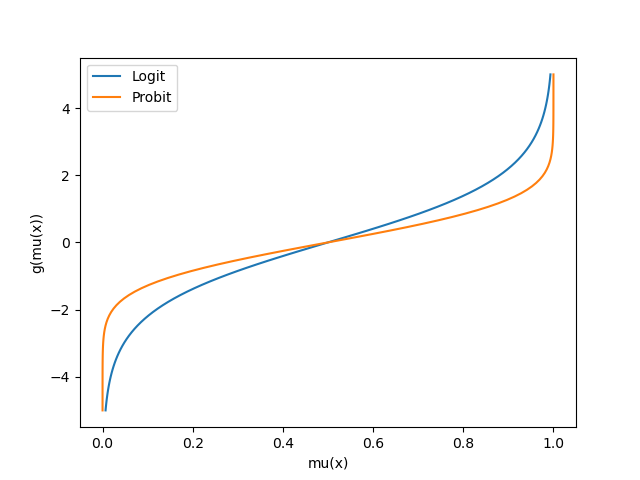
\includegraphics[scale=0.5]{img/probit_logit.png}
            \caption{Logit and Probit Functions}
            \label{fig:logit_probit}
        \end{figure}
    \end{enumerate}
    \end{example}

    Now there are many choices of functions we can take. In fact, if $\mu$ lives in $(0, 1)$, then we can really just take our favorite distribution that has a density that is supported everywhere in $\mathbb{R}$ and take the inverse cdf as our link. So far, we have no reason to prefer one function to another, but in the next section, we will see that there are more natural choices. 

    \subsubsection{Canonical Link Functions}

      Now let's summarize what we have. We assume that the conditional distribution $Y \mid X = x$ follows a distribution in the exponential family, which we can completely characterize by the cumulant generating function $\psi$. For different values of $x$, the conditional distribution will be paramaterized by different $\eta (x)$, and the resulting distribution $P_\eta$ will have some mean $\mu(x)$, which is usually not the natural parameter $\eta$. Now, let's forget about our knowledge that $\psi^\prime(\eta) = \mu$, but we know that there is some relationship between $\eta \leftrightarrow \mu$.

      Given an $x$, I need to use the linear predictor $x^T \beta$ to predict $\mu(x)$, which can be done through the link function $g$. 
      \[g\big( \mu(x) \big) = x^T \beta\]
      Now what would be a natural way of choosing this $g$? Note that our natural parameter $\eta$ for this canonical family takes value on the entire real line. I must construct a function $g$ that maps $\mu$ onto the entire real line, and so why not make it map to $\eta$. Therefore, we have 
      \[\eta(x) = g\big( \mu(x) \big) = x^T \beta\]

      \begin{definition}[Canonical Link]
      The function $g$ that links the mean $\mu$ to the canonical parameter $\theta$ is called the \textbf{canonical link}. 
      \[g(\mu) = \theta\]
      Now using our knowledge that $\psi^\prime(\eta) = \mu$, we can see that 
      \[g = (\psi^\prime)^{-1}\]
      This is indeed a valid link function. 
      \begin{enumerate}
          \item $\psi^{\prime\prime} > 0$ since it models the variance, and so $\psi^\prime$ is strictly increasing and so $g = (\psi^\prime)^{-1}$ is also strictly increasing. 
          \item The domain of $\psi^\prime$ is the real line since it takes in the natural parameter $\eta$ which exists over $\mathbb{R}$, so $\mathrm{Im}(g) = \mathbb{R}$. 
      \end{enumerate}
      \end{definition}

      So, given our cumulant generating function $\psi$ and our link function $g$, both satisfying 
      \[\psi^\prime (\eta) = \mu \text{ and } g(\mu) = x^T \beta\]
      we can combine them to get 
      \[(g \circ \psi^\prime) (\eta) = g(\mu) = x^T \beta\]
      and so, even though the mean of the response variable is not linear with respect to $x$, the value of $(g \circ \psi^\prime) (\eta)$ is indeed linear. In fact, if we choose the canonical link, then the equation 
      \[\eta = x^T \beta\]
      means that the natural parameter of our conditional distribution in the exponential family is linear with respect to $x$! From this we can find the conditional mean $\mu(x)$. 

      The reason we focus on canonical link functions is because, when the canonical link is used, the components of the model (the parameters of the linear predictor) have an additive effect on the response variable in the transformed (linked) scale, which makes the interpretation of the results easier. It's also worth noting that while using the canonical link function has some desirable properties, it is not always the best or only choice, and other link functions may be used if they provide a better fit for the data or make more sense in the context of the problem at hand.

      Let us evaluate some canonical link functions. 

      \begin{example}
      The Bernoulli has the canonical exponential form of 
      \[p_\eta (x) = \exp \big[ x \eta - \log (1 + e^\eta) \big]\]
      where $\eta = \log \big( \frac{\theta}{1 - \theta} \big)$. Since we have prior knowledge that $\theta = \mu$ (i.e. the expectation of a Bernoulli is the hyperparameter $\theta$ itself), we have a function that maps $\mu \mapsto \eta$. 
      \[\eta = g(\mu) = \log \bigg( \frac{\mu}{1 - \mu} \bigg)\]
      which gives us our result. We can also take the inverse of $\psi^\prime = \frac{e^\eta}{1 + e^\eta}$ to get our result 
      \[g (\mu) = (\psi^\prime)^{-1} (\mu) = \log \bigg( \frac{\mu}{1 - \mu} \bigg) \]
      \end{example}

  \subsection{Likelihood Optimization}

    Now let us have a bunch of data points $\{(x_n, y_n)\}_{n=1}^N$. By our model assumption, we know that the conditional distribution $Y \mid X = x_n$ is now of an exponential family with parameter $\eta_n = \eta (x_n)$ and density 
    \[p_{\eta_n} (y_n) = \exp \big[ y_n \eta_n - \psi(\eta_n) \big] h(y_n)\]
    Now we want to do likelihood optimization on $\beta$ (not $\eta$ or $\mu$), and to do this, we must rewrite the density function in a way so that it depends on $\beta$. Given a link function $g$, note the following relationship between $\beta$ and $\eta$: 
    \begin{align*}
        \eta_n = \eta (x_n) & = (\psi^\prime)^{-1} (\mu (x_n)) \\
        & = (\psi^{\prime})^{-1} \big( g^{-1} (x_n^T \beta )\big) \\
        & = h(x_n^T \beta) 
    \end{align*}
    where for shorthand notation, we define $h \coloneqq (g \circ \psi^\prime)^{-1}$. Subtituting this into the above likelihood, taking the product of all $N$ samples, and logarithming the equation gives us the following log likelihood to optimize over $\beta$. 
    \[\ell(\beta) = \log \prod_{n=1}^N p_{\eta_n} (y_n) = \sum_{n=1}^N y_n h(x_n^T \beta)  - \psi(h(x_n^T \beta) )\]
    where we dropped the $h(y_n)$ term at the end since it is a constant and does not matter. If $g$ was the canonical link, then $h$ is the identity, and we should have a linear relationship between $\eta (x_n) = x_n^T \beta$. This means that the $\eta_n$ reduces only to $x_n^T \beta$, which is much more simple to optimize. 
    \[\ell(\beta) = \log \prod_{n=1}^N p_{\eta_n} (y_n) = \sum_{n=1}^N y_n x_n^T \beta - \psi(x_n^T \beta)\]
    Note that the first term is linear w.r.t $\beta$, and $\psi$ is convex, so the entire sum must be concave w.r.t. $\beta$. With this, we can bring in some tools of convex optimization to solve. 

\section{Boosting} 

  \subsection{AdaBoost} 

  \subsection{XGBoost}

  \subsection{Random Forests}

\section{Bagging}

\section{Density Estimation}

  \subsection{Kernel Density Estimation} 

\section{Clustering and Density Estimation} 

  \subsection{K Means} 

  \subsection{Mixture Models}

  \subsection{Density Based Clustering}

  \subsection{Hierarchical Clustering} 

  \subsection{Spectral Clustering}

  \subsection{High Dimensional Clustering}

\section{Graphical Models} 

  \subsection{Bayesian Networks} 

  \subsection{Markov Random Fields}

  \subsection{Hidden Markov Models}

\section{Dimensionality Reduction} 

  \subsection{Random Matrix Theory} 

  \subsection{Factor Analysis}

  \subsection{Sparse Dictionary Learning}

  \subsection{Principal Component Analysis} 

  \subsection{Independent Component Analysis} 

  \subsection{Latent Dirichlet Allocation} 

  \subsection{UMAP}

  \subsection{t-SNE}


\end{document}
